% This is the report Template for Fr. C Rodrigues Institute of Technology, Vashi

% Authored by -  Dr. Smita Dange

% Modularised every section into different .tex files

% This is the preamble.  

% Any package you would like to use, please add it to this .tex and not the other .tex files because if you do...the code will not compile! Other .tex files are only for filing content. Any styling has to happen in this file.

% Good Luck!

\documentclass[12pt]{report}
\usepackage{hyperref}
\usepackage{kantlipsum}
\usepackage{graphicx}
\usepackage{geometry}
\usepackage{ragged2e}
\usepackage{titlesec}
\usepackage{fancyhdr}
\usepackage{tabularx}
\usepackage{array}

\titleformat{\chapter}[display]
  {\normalfont\huge\bfseries\centering}
  {\chaptertitlename\ \thechapter}{24pt}{\Huge}
\geometry{verbose,a4paper,tmargin=15mm,bmargin=30mm,lmargin=30mm,rmargin=20mm}

%creating a user defined footer and header
\geometry{headheight=15pt}
\setcounter{tocdepth}{3}
\setcounter{secnumdepth}{3}

\pagestyle{fancy}
\fancyhf{}
\rhead{Agentic AI Procurement Solution }
\lfoot{F.C.R.I.T, Vashi}
\rfoot{\thepage}
\renewcommand{\footrulewidth}{0.6pt}
\renewcommand{\headrulewidth}{1.pt}

\begin{document}
\pagestyle{plain}
%Title Page

\begin{titlepage}
%%%% \pagenumbering{gobble}
\thispagestyle{empty}

{\centering
{A Project Report}\\ 
\vspace{0.2cm}
{On}
\vspace{0.3cm}
\\
}
 
{\centering
\large

{\LARGE\bf Agentic AI Procurement Solution}\\
\vspace{1cm}
{Submitted in partial fulfilment of the requirements of } \\
\vspace{0.2cm}
{\bf{University of Mumbai}} \\
\vspace{0.2cm}
{For the Degree of} \\
\vspace{0.2cm}
{\bf {Bachelor of Engineering }} \\
{\it{in}} \\
{\bf COMPUTER ENGINEERING } \\
\vspace{0.5cm}
\it{Submitted by} \\
\vspace{.2cm}
\rm
{\large \bf {More Anjali Dinesh}}\\
{\large \bf {Sankaye Vaidehi Jagdeep}}\\
{\large \bf {Sawant Niraj Ravindra}}\\
{\large \bf {Shete Anooj  }}\\

\vspace{0.8 cm}
{\it{Supervised by}} \\
\vspace{.1cm}
\hspace{.05cm} {\large \textbf {Dr. Jyoti More}}\\
\vspace{0.1cm}
{\it{\&}} \\
\vspace{.1cm}
\hspace{.02cm} {\large \textbf {Mr. Alok}}\\
\vspace{.05cm}
\hspace{.01cm} {\large \textbf {(External guide)}}\\


\vspace {0.4cm}




\begin{figure}[h]
{\centering {
\includegraphics[width=4cm,height=4cm]{fcritlogo}}\par}
\end{figure}

{\bf Department of Computer Engineering \\
\vspace{0.1cm}
\bf {Fr. Conceicao Rodrigues Institute of Technology}\\
\bf{ An Autonomous Institute \& Permanently Affiliated to University of Mumbai}
\bf Sector 9A, Vashi, Navi Mumbai - 400703} \\
{\centering
\hspace{.2cm}


{\centering
{\bf UNIVERSITY OF MUMBAI} \\
\bf{ 2026-2027 } \\
}

}\end{titlepage} 
\pagenumbering{roman}


%\pagenumbering{gobble}

% Approval Page 

\begin{center}

{\LARGE\bf APPROVAL SHEET}

\vspace{1cm}

{\large This is to certify that the project entitled}\\[0.3cm]

{\Large\bf \textsc{Agentic AI Procurement Solution}\\[0.3cm]

{\large\bf Submitted by}\\[0.5cm]

\begin{table}[h]
\centering
\Large
\begin{tabular}{cc}
\textbf{More Anjali Dinesh} & \textbf{1023207} \\
\textbf{Sankaye Vaidehi Jagdeep} & \textbf{1023239} \\
\textbf{Sawant Niraj Ravindra} & \textbf{1023240} \\
\textbf{Shete Anooj} & \textbf{1023250}

\end{tabular}
\end{table}

\vspace{2cm}

%------------------------------------------------
% Supervisor and Project Coordinator
%------------------------------------------------

\begin{tabular}{cc}
\begin{minipage}{0.42\textwidth}
\centering
\rule{5cm}{0.2px}\\
\textbf{Supervisor / Project Guide}
\end{minipage}
&
\begin{minipage}{0.42\textwidth}
\centering
\rule{5cm}{0.2px}\\
\textbf{Project Coordinator}
\end{minipage}
\end{tabular}

\vspace{2.2cm}

%------------------------------------------------
% Internal and External Examiner
%------------------------------------------------

\begin{tabular}{cc}
\begin{minipage}{0.42\textwidth}
\centering
\rule{5cm}{0.2px}\\
\textbf{Internal Examiner}
\end{minipage}
&
\begin{minipage}{0.42\textwidth}
\centering
\rule{5cm}{0.2px}\\
\textbf{External Examiner}
\end{minipage}
\end{tabular}

\vspace{2.2cm}

%------------------------------------------------
% HOD and Principal
%------------------------------------------------

\begin{tabular}{cc}
\begin{minipage}{0.42\textwidth}
\centering
\rule{5cm}{0.2px}\\
\textbf{Head of Department}
\end{minipage}
&
\begin{minipage}{0.42\textwidth}
\centering
\rule{5cm}{0.2px}\\
\textbf{Principal}
\end{minipage}
\end{tabular}

\vspace{1.5cm}

%------------------------------------------------
% College Seal
%------------------------------------------------

\textbf{COLLEGE SEAL}

\vspace{2cm}

\begin{flushleft}
\textbf{Date :} \rule{4cm}{0.2px}\\[0.4cm]
\textbf{Place :} \rule{4cm}{0.2px}
\end{flushleft}

\end{center}


% Declaration Page

\begin{centering}
\large
{\LARGE\bf Declaration}\\
\end{centering}

% workaround for the inconsistent justify. If someone figures out the right way to strictly justify, let me know
\justify
We declare that this written submission for B.E. Declaration entitled \\
"{\bf Agentic AI Procurement Solution}" represents our ideas in our own words and where others' ideas or words have been included. We have adequately cited and referenced the sources. We also declare that we have adhered to all principles of academic honesty and integrity and have not misrepresented, fabricated, or falsified any ideas/data/fact/source in our submission. We understand that any violation of the above will cause disciplinary action by the institute and also evoke penal action from the sources which have thus not been properly cited or from whom permission has not been taken when needed.  \\ 

\vspace{3cm}
\hfill% move it to the right
\begin{tabular}[t]{l@{}}
\vspace{1cm}

{\textbf{Project Group Members:}} \\ 
\vspace{1cm}

1. More Anjali Dinesh, 1023207 \\
\noindent\rule{5cm}{0.10pt} \\
\\
\vspace{1cm}

2. Sankaye Vaidehi Jagdeep, 1023239 \\
\noindent\rule{5cm}{0.10pt} \\
\\
\vspace{1cm}

3. Sawant Niraj Ravindra, 1023240 \\
 \noindent\rule{5cm}{0.10pt}
\\
\vspace{1cm}


4. Shete Anooj, 1023250 \\
 \noindent\rule{5cm}{0.10pt}

\end{tabular}

%%%%%%%%%%%%%%%%%%%%%%%%%%%%%%%%%%%%IGNORE PLEASE !
%\begin{flushright} 
%\vspace{0.5in}
%\noindent\rule{4cm}{0.4pt} \\ (Signature)\\
%\vspace{0.3in}
%\noindent\rule{4cm}{0.4pt} \\ (Name of the Student)
%\end{flushright}
%\vspace{0.5cm}
%{\bf Date:} \\
%%%%%%%%%%%%%%%%%%%%%%%%%%%%%%%%%%%%


%% End of Declaration Page


% Table of Contents
\newpage

%Abstract
\addcontentsline{toc}{chapter}{Abstract}
% Abstract Page
\vspace{1in}
\chapter*{Abstract}


IT procurement is an important activity in organizations involved in the purchase, licensing, renewal and risk assessment of IT resources. The conventional procurement process involves manual checks, spreadsheets, emails and multiple systems leading to slow down, procurement of the same items, unused licences and blind spots about vendor risk.A variety of techniques including rule-based, document intensive, OCR, machine learning, and approval automation techniques can be employed to improve procurement processes but individual techniques typically focus on one or more stages in the procurement cycle but are limited in providing an end-to-end view of procurement activities. As a result, there is a need to develop a system that helps procure IT resources by orchestrating multiple procurement activities with minimal human intervention.
The application of Agentic AI is appropriate in this scenario as multiple specialised agents can be deployed to execute and coordinate various functions
In this paper, an Agentic AI-Based IT Procurement Intelligence Platform is designed based on a modular event driven monolithic architecture. The architecture comprises document and vendor intelligence agents, approval and inventory agents, contract and risk intelligence agents and the platform core services which operate on the principles of Apache Kafka, FastAPI, PostgreSQL, Redis and React technologies. Document processing techniques including OCR, classification and information extraction are deployed for purchase order, invoice and vendor quotation processing while machine learning techniques are applied in detecting duplicate purchases, analysing utilisation of licences and assessing vendor risk. The system integrates information and automates a variety of procurement activities with human agent involvement for low confidence and high priority items. The expected outcome of the developed system is to reduce the manual processing of procurement activities, improve procurement process efficiency, reduce unwarranted procurement expenditures and provide insights on vendor and procurement risks.

\tableofcontents
\newpage

\addcontentsline{toc}{chapter}{List of Figures}
\listoffigures
\newpage

\addcontentsline{toc}{chapter}{List of Tables}
\listoftables
\newpage

\newpage

\pagenumbering{arabic}

\pagestyle{fancy}
% Chapter 1 Introduction

\chapter[Introduction]{\centering Introduction}\label{chap1}
\newpage

\section{Background}
IT procurement is an important part of an organization’s operations as it involves the acquisition and management of hardware, software licenses, SaaS subscriptions, and related services. The procurement process involves several stages including vendor identification, document processing, approval, inventory management, contract handling and vendor risk assessment. In many organizations, these activities are handled through emails, spreadsheets, invoices, and separate systems, making it challenging to maintain a consistent and updated view of procurement activities. As a result, approvals can be delayed, purchases duplicated and licenses left unused, difficulties with tracking contracts and increased vendor-related risks. The opportunity to use artificial intelligence and automation presents an opportunity to improve these activities and make the procurement process more efficient.


\section{Motivation}
The rationale behind the project revolves around the need to reduce the amount of time spent on IT procurement manual processes as well as increase transparency and control during the procedure. Currently, several steps have to be taken by employees in the process, including verifying documents, reviewing vendor details, requesting and obtaining approvals, checking the utilisation of inventory, and ensuring the renewal of contracts among other aspects. These procedures create difficulties, especially when the data involved is high in volume, and a system that can help automate and optimise processing and support cross-functional communication would be of great benefit. The project, therefore, aims to implement a set of special-purpose software agents that will utilise artificial intelligence to assist with document processing, vendor identification, approvals, inventory use analysis, contract management, and risk detection among other fields.
\section{Aim and Objectives}

\subsection{Aim}

To develop an \textbf{Agentic AI-Based IT Procurement Intelligence Platform} that integrates, automates, and intelligently manages major activities involved in the IT procurement lifecycle while maintaining human oversight for critical decisions.

\subsection{Objectives}

\begin{itemize}
    \item To process and extract relevant information from procurement documents such as purchase orders, invoices, and quotations.
    
    \item To verify vendor information and identify duplicate vendors and invoices.
    
    \item To automate approval workflows based on spending limits, budgets, user roles, and inventory availability.
    
    \item To identify underutilised software licenses and support their controlled reclamation.
    
    \item To assist in contract management and monitor important renewal-related information.
    
    \item To continuously assess vendor-related risks using machine learning techniques.
    
    \item To provide shared platform services such as notifications, authentication, monitoring, and system management.
    
    \item To maintain human involvement in low-confidence results and critical procurement decisions.
\end{itemize}

\section{Problem statement}


IT procurement involves several activities such as collecting procurement documents, verifying vendor information, processing invoices and quotations, obtaining approvals, managing software licenses, monitoring contracts, and assessing vendor risks. These activities are often handled through multiple systems and manual processes, resulting in delays, duplicate records, inefficient resource utilisation, and limited visibility across the procurement lifecycle.

Traditional procurement systems primarily focus on recording and managing transactions rather than intelligently analysing procurement data and assisting users in decision-making. Identifying duplicate vendors or invoices, detecting underutilised software licenses, tracking contract renewals, and assessing vendor-related risks may require significant manual effort. Furthermore, automated decisions without proper confidence assessment and human oversight can lead to incorrect procurement actions.

Therefore, there is a need for an intelligent and integrated solution that can automate routine procurement activities, analyse relevant data, assist in approval and decision-making processes, and continuously monitor procurement-related risks. The proposed Agentic AI-Based IT Procurement Intelligence Platform aims to address these challenges by integrating AI-driven analysis, workflow automation, document processing, vendor intelligence, license management, contract monitoring, and human-in-the-loop mechanisms within a unified platform.

\section{Scope}

The scope of the proposed Agentic AI-Based IT Procurement Intelligence Platform includes the development of an integrated system to support major activities involved in the IT procurement lifecycle. The platform will focus on the following areas:

\begin{itemize}
    \item \textbf{Procurement Document Processing:} Processing purchase orders, invoices, quotations, and other relevant procurement documents to extract and structure important information.

    \item \textbf{Vendor Intelligence:} Verifying vendor information, identifying duplicate vendors, and maintaining relevant vendor records.

    \item \textbf{Invoice and Duplicate Detection:} Analysing invoice information to identify duplicate or potentially inconsistent records.

    \item \textbf{Approval Workflow Automation:} Supporting procurement approval workflows based on predefined spending limits, budgets, user roles, and inventory availability.

    \item \textbf{Software License Management:} Identifying underutilised software licenses and supporting their controlled reclamation or reassignment.

    \item \textbf{Contract Management:} Maintaining contract-related information and monitoring important dates, including contract renewal and expiration.

    \item \textbf{Vendor Risk Assessment:} Applying machine learning techniques to analyse vendor-related information and continuously assess potential risks.

    \item \textbf{Shared Platform Services:} Providing common services such as authentication, notifications, monitoring, logging, and system management.

    \item \textbf{Human-in-the-Loop Decision Making:} Routing low-confidence results and critical procurement decisions to authorised users for review and approval.

    \item \textbf{Agentic AI Integration:} Using AI agents to coordinate relevant procurement tasks, analyse information, and assist users across different stages of the procurement lifecycle.
\end{itemize}

The platform is intended to assist procurement teams by reducing manual effort, improving data accuracy, increasing process visibility, and supporting informed decision-making. The system will focus on decision support and workflow automation rather than completely replacing human decision-makers in critical procurement activities.
```

\section{Report Outline}



This report is organized into six chapters. Chapter 1, \textbf{Introduction}, presents the background and motivation of the project, followed by the aim and objectives, problem statement, scope, and report outline. Chapter 2, \textbf{Study of the System}, discusses the techniques relevant to the proposed system, various available techniques, and related works in the field of IT procurement and Agentic AI. Chapter 3, \textbf{Proposed System}, describes the problem addressed by the project, its scope, and the proposed Agentic AI-Based IT Procurement Intelligence Platform. Chapter 4, \textbf{Design of the System}, covers requirement engineering, requirement elicitation, software lifecycle model, requirement analysis, UML diagrams and DFDs, cost analysis, hardware and software requirements, system architecture, UI/UX design, and the block diagram of the system. Chapter 5, \textbf{Result and Discussion}, presents the implemented system through screenshots, important code and main logic, and discusses the testing performed, including unit testing, integration testing, and black-box testing. Chapter 6, \textbf{Conclusion and Future Scope}, summarizes the project outcomes, limitations, and possible future enhancements. The report also includes references and appendices covering the project timeline, SDG mapping, complex engineering problem identification and evaluation, and project outcomes.




%%%% End of Chapter 1
% ============================================================
% Chapter 2: Literature Review (drop-in chapter file)
% Needs NO extra packages: plain LaTeX tables only.
% ============================================================

\chapter{Study of the System} \label{chap2}
\newpage

Procurement departments handle a steady stream of documents, including purchase orders, invoices and vendor quotations, and these rarely arrive in the same form twice. Some come by email, some through vendor portals, and others are scans of printed pages. In many organisations someone still reads each one and types the details into a system by hand. Contracts are followed up in spreadsheets, vendors are vetted once at onboarding, and software licenses are checked with a simple inactivity rule. Over time this leads to typing mistakes, duplicate payments, vendors whose identity was never properly confirmed, contracts that renew without anyone noticing, and licenses that are paid for but never used. Fraud is a further concern. In Business Email Compromise (BEC), an attacker poses as a supplier and asks for bank details to be changed, and the request goes through because nobody verifies it independently.

This work studies a platform that tackles these problems through four agents communicating over events: Document and Vendor Intelligence, Approval and Inventory Intelligence, Contract and Risk Analysis, and a Platform agent for notifications, authentication and monitoring. Because each agent relies on a different set of techniques, the chapter covers a range of methods instead of a single one. It begins with how procurement is traditionally done and where that approach falls short, and then reviews the main techniques for each part of the problem, noting the strengths and weaknesses of each. Ten related research works are then compared, and the chapter ends with a summary of the literature and the gap this project sets out to address.

\section{About the Technique}

Traditional procurement processing rests on four habits. The first is manual or template-based data entry: staff key in invoice and purchase order details, or an OCR template is built for each vendor's layout. The second is static approval rules, where a request follows a fixed chain with no deadline, no escalation and no awareness of the remaining budget. The third is periodic vendor review, which in practice often means one questionnaire at onboarding. The fourth is the flat-threshold license audit, in which a seat is flagged if nobody has logged in for some fixed number of days.

These habits work well enough when volumes are small, but they break down quickly as an organisation grows. Table~\ref{tab:traditional} summarises where each of them struggles.

\begin{table}[!htbp]
\centering
\footnotesize
\renewcommand{\arraystretch}{1.2}
\caption{Traditional procurement practices and their shortcomings}
\label{tab:traditional}
\begin{tabular}{|p{\dimexpr 0.20\textwidth-2\tabcolsep\relax}|p{\dimexpr 0.28\textwidth-2\tabcolsep\relax}|p{\dimexpr 0.50\textwidth-2\tabcolsep\relax}|}
\hline
\raggedright \textbf{Area} & \raggedright \textbf{Traditional approach} & \raggedright \textbf{Shortcoming} \tabularnewline \hline
\raggedright Data capture & \raggedright Manual entry and per-vendor templates & \raggedright Slow and error-prone; needs updating whenever a vendor changes its document layout. \tabularnewline \hline
\raggedright Vendor verification & \raggedright Manual lookup and email confirmation & \raggedright Vulnerable to Business Email Compromise (BEC) fraud and duplicate vendor records. \tabularnewline \hline
\raggedright Approvals & \raggedright Email chains and fixed rules & \raggedright No SLA timers or escalation; conflicts in budget allocation and stock availability. \tabularnewline \hline
\raggedright License management & \raggedright Fixed inactivity threshold & \raggedright Ignores usage patterns and may wrongly flag seasonal drops in activity. \tabularnewline \hline
\raggedright Contract tracking & \raggedright Calendar reminders & \raggedright Notice periods may be missed, resulting in unintended automatic renewals. \tabularnewline \hline
\raggedright Risk assessment & \raggedright One-time questionnaire & \raggedright Becomes outdated and may miss new sanctions or adverse news. \tabularnewline \hline
\end{tabular}
\end{table}

These gaps are what motivate an automated, event-driven approach. The idea is not to hand everything to a model. Pretrained models handle the perception-heavy work such as reading documents and clauses, a small amount of custom training is used where a task is specific to this project, and plain rules are kept for the places where certainty matters, such as a sanctions match.

\section{Various Available Techniques}

\subsection{Document Intelligence}
Template-based and regular-expression approaches are quick and predictable, but they are brittle when vendors change their layouts. OCR engines such as Tesseract and PaddleOCR can extract text from scanned documents, but they lose table structure in the process. Layout-aware parsers such as Docling recover the reading order and table structure of a document, but are not optimised for invoices. Multimodal transformers, particularly those in the LayoutLM family, achieve the best results on forms and invoices, but they need labelled data to fine-tune and more compute to run. This project uses Docling (with PaddleOCR for scanned pages) as the primary pipeline and runs LayoutLMv3 as an independent cross-check, routing any disagreement to human review.

\subsection{Document Classification}
TF-IDF with logistic regression is light, fast to train and easy to inspect, which makes it a good choice for a three-class problem (PO, invoice, quote). It ignores word order and layout and depends on the quality of the training data. Transformer classifiers such as BERT have a higher ceiling but need more data and compute than this task justifies.

\subsection{Vendor Deduplication and Identity Verification}
Fuzzy name matching (rapidfuzz) tolerates spelling differences but can produce false matches when used on its own. Official identifiers such as GSTIN and IFSC are more reliable, but live lookups are limited by API quotas. ClamAV scans files on upload using signature-based detection, which is quick but offers no protection against zero-day threats.

\subsection{Workflow Orchestration and Concurrency Control}
Cron jobs and scripts are simple to set up, but they are not durable and do not handle deadlines. Temporal offers timers, escalation and replay, but has a steeper learning curve. Redis locks and database-level locks stop two requests from claiming the same stock or budget at once, but need careful handling of failures. Kafka provides decoupled, replayable events between agents, provided the consumers are idempotent.

\subsection{Usage Anomaly Detection and Explainability}
A flat inactivity threshold is transparent but flags seasonal and weekend dips by mistake. Isolation Forest is unsupervised and efficient on tabular data, though it is sensitive to the contamination setting and has no built-in explanations. SHAP supplies per-license feature contributions at some extra computational cost.

\subsection{Contract Analysis and Clause Extraction}
Keyword search misses paraphrased clauses. Legal-BERT fine-tuned on CUAD handles legal wording better and answers one question per field, but it was trained mostly on US-style contracts and can only extract text that exists. FinBERT scores financial sentiment in adverse media, although sentiment is only a rough proxy for risk.

\subsection{Vendor Risk Scoring and Drift Monitoring}
Static questionnaires are only snapshots, whereas a learned classifier can combine continuous signals, and hard-override rules force a High band for facts such as a sanctions match or a cancelled GSTIN. Sanctions screening uses fuzzy matching on the OpenSanctions dataset with tuned thresholds. The Population Stability Index warns of model drift but does not retrain the model.

\subsection{Multi-Agent and Agentic Architectures}
Splitting the workflow among specialised agents gives modularity and clear ownership, at the cost of integration effort. This platform manages that through a shared event contract, correlation-ID tracing, common authentication middleware and a quota-managed Live Verification Mode.

\section{Related Works}

To see where this system fits, we looked at ten published works, each covering one building block of the platform. They are grouped below by the problem they address, and Table~\ref{tab:related} then puts them side by side.

\paragraph{Document understanding.} LayoutLM~\cite{xu2020layoutlm} was among the first models to learn from text and its two-dimensional position on the page together, and it improved results on forms, receipts and invoices considerably. Its successor, LayoutLMv3~\cite{huang2022layoutlmv3}, added image information through a shared text-and-image masking objective and dropped the CNN backbone, giving a simpler and stronger model. On the tooling side, Docling~\cite{auer2024docling} offers an open-source pipeline that rebuilds reading order and table structure locally, and PaddleOCR~3.0~\cite{cui2025paddleocr} provides accurate multilingual OCR with structure analysis, although it runs best on a GPU.

\paragraph{Contract and risk language.} CUAD~\cite{hendrycks2021cuad} gives 510 expert-annotated contracts covering 41 clause types, and has become the standard benchmark for clause extraction. LEGAL-BERT~\cite{chalkidis2020legalbert} showed that pretraining on legal text clearly outperforms generic BERT on legal tasks. For the financial side of vendor risk, FinBERT~\cite{araci2019finbert} contributes sentiment analysis tuned to financial language.

\paragraph{Anomaly detection and explanation.} Isolation Forest~\cite{liu2008isolation} finds unusual records by how quickly random splits separate them from the rest, so it needs no labelled examples. SHAP~\cite{lundberg2017shap} then explains a single prediction by showing how much each feature pushed the score up or down.

\paragraph{Agent frameworks.} AutoGen~\cite{wu2023autogen} stands for the popular LLM-driven approach in which agents cooperate by conversation. We include it mainly as a contrast to the design chosen here.

\begin{table}[!htbp]
\centering
\footnotesize
\sloppy
\renewcommand{\arraystretch}{1.2}
\caption{Comparison of related works}\label{tab:related}
\begin{tabular}{|p{\dimexpr 0.17\textwidth-2\tabcolsep\relax}|p{\dimexpr 0.22\textwidth-2\tabcolsep\relax}|p{\dimexpr 0.19\textwidth-2\tabcolsep\relax}|p{\dimexpr 0.20\textwidth-2\tabcolsep\relax}|p{\dimexpr 0.20\textwidth-2\tabcolsep\relax}|}
\hline
\raggedright \textbf{Reference} & \raggedright \textbf{Contribution} & \raggedright \textbf{Advantages} & \raggedright \textbf{Limitations} & \raggedright \textbf{Role in this system} \tabularnewline \hline
\raggedright Xu et al., LayoutLM (KDD 2020) \cite{xu2020layoutlm} & \raggedright Joint pretraining of text and 2D layout for document images & \raggedright Large gains on forms, receipts and invoices & \raggedright No image features in pretraining; needs fine-tuning & \raggedright Foundation of the LayoutLMv3 fallback \tabularnewline \hline
\raggedright Huang et al., LayoutLMv3 (ACM MM 2022) \cite{huang2022layoutlmv3} & \raggedright Unified text-image masking, no CNN backbone & \raggedright State-of-the-art results; simpler architecture & \raggedright Compute-heavy; needs labels for new document types & \raggedright Independent cross-check extraction path \tabularnewline \hline
\raggedright Auer et al., Docling (2024) \cite{auer2024docling} & \raggedright Open-source layout, reading-order and table recovery & \raggedright Fast, local, strong on tables & \raggedright Not tuned to invoices; weak on poor scans & \raggedright Primary layout parser \tabularnewline \hline
\raggedright Cui et al., PaddleOCR 3.0 (2025) \cite{cui2025paddleocr} & \raggedright OCR and structure-analysis toolkit (PP-StructureV3) & \raggedright Accurate, multilingual & \raggedright GPU preferred; errors on low-quality scans & \raggedright OCR for image-only pages \tabularnewline \hline
\raggedright Hendrycks et al., CUAD (NeurIPS 2021) \cite{hendrycks2021cuad} & \raggedright 510 contracts, 41 clause categories & \raggedright Realistic benchmark, CC BY 4.0 & \raggedright English, mostly US contracts & \raggedright Benchmark for clause extraction \tabularnewline \hline
\end{tabular}
\end{table}

\begin{table}[!htbp]
\centering
\footnotesize
\sloppy
\renewcommand{\arraystretch}{1.2}
\caption{Comparison of related works (continued)}
\begin{tabular}{|p{\dimexpr 0.17\textwidth-2\tabcolsep\relax}|p{\dimexpr 0.22\textwidth-2\tabcolsep\relax}|p{\dimexpr 0.19\textwidth-2\tabcolsep\relax}|p{\dimexpr 0.20\textwidth-2\tabcolsep\relax}|p{\dimexpr 0.20\textwidth-2\tabcolsep\relax}|}
\hline
\raggedright \textbf{Reference} & \raggedright \textbf{Contribution} & \raggedright \textbf{Advantages} & \raggedright \textbf{Limitations} & \raggedright \textbf{Role in this system} \tabularnewline \hline
\raggedright Chalkidis et al., LEGAL-BERT (EMNLP 2020) \cite{chalkidis2020legalbert} & \raggedright BERT pretrained on legal corpora & \raggedright Beats generic BERT on legal tasks & \raggedright Smaller corpus; mostly English & \raggedright Base of the Legal-BERT-CUAD extractor \tabularnewline \hline
\raggedright Araci, FinBERT (2019) \cite{araci2019finbert} & \raggedright BERT further pretrained on financial text & \raggedright Strong financial sentiment & \raggedright Sentiment is only a proxy for risk & \raggedright Adverse-media signal in risk score \tabularnewline \hline
\raggedright Liu et al., Isolation Forest (ICDM 2008) \cite{liu2008isolation} & \raggedright Anomaly detection by random partitioning & \raggedright Linear time, no labels, high-dimensional data & \raggedright No native explanation; contamination must be set & \raggedright License-usage anomaly scoring \tabularnewline \hline
\raggedright Lundberg and Lee, SHAP (NeurIPS 2017) \cite{lundberg2017shap} & \raggedright Unified feature attribution & \raggedright Consistent local explanations; fast for trees & \raggedright Cost grows with features; not causal & \raggedright Top factors behind each anomaly score \tabularnewline \hline
\raggedright Wu et al., AutoGen (2023) \cite{wu2023autogen} & \raggedright Multi-agent LLM conversation framework & \raggedright Modular and customisable & \raggedright Conversation-driven; hard to audit & \raggedright Contrast: we use event-driven agents with durable workflows \tabularnewline \hline
\end{tabular}
\end{table}


Taken together, the works show a clear pattern. The document-AI papers are mainly about how accurately fields can be read, and they say little about what should happen next, such as verifying the vendor, catching duplicates or blocking fraud. This platform adds a fail-closed pipeline around that extraction step. The legal NLP papers stop at pulling clauses out of text, while here the extracted terms sit in the same system as a live risk score, where hard overrides take priority over the learned model. Isolation Forest and SHAP are general-purpose tools, so the new part is how they are applied to software-license reclaim, with a grace period and cooldown that treat users fairly. Finally, agent frameworks like AutoGen prioritise flexibility and free-form dialogue, whereas procurement needs predictable, auditable and concurrency-safe behaviour. That is why we rely on Kafka~\cite{kreps2011kafka} for events and Temporal-style workflows for orchestration.

\section{Literature Summary and Research Gap}

Table~\ref{tab:summary} pulls together the techniques reviewed and shows where each one is used in the proposed system.

\begin{table}[!htbp]
\centering
\small
\renewcommand{\arraystretch}{1.25}
\caption{Techniques reviewed and their use in the proposed system}
\label{tab:summary}
\begin{tabular}{|p{\dimexpr 0.22\textwidth-2\tabcolsep\relax}|p{\dimexpr 0.34\textwidth-2\tabcolsep\relax}|p{\dimexpr 0.42\textwidth-2\tabcolsep\relax}|}
\hline
\raggedright \textbf{Area} & \raggedright \textbf{Best-known technique} & \raggedright \textbf{Use in this system} \tabularnewline \hline
\raggedright Layout and OCR & \raggedright Docling, PaddleOCR & \raggedright Primary extraction pipeline \tabularnewline \hline
\raggedright Extraction cross-check & \raggedright LayoutLMv3 & \raggedright Fallback path with human review \tabularnewline \hline
\raggedright Classification & \raggedright TF-IDF + logistic regression & \raggedright Trained from scratch, tracked in MLflow \tabularnewline \hline
\raggedright Clause extraction & \raggedright Legal-BERT on CUAD & \raggedright Renewal type, notice period, end date \tabularnewline \hline
\raggedright Anomaly detection & \raggedright Isolation Forest + SHAP & \raggedright License reclaim scoring \tabularnewline \hline
\raggedright Risk scoring & \raggedright Classifier + rule overrides + FinBERT & \raggedright Risk bands; sanctions as hard override \tabularnewline \hline
\raggedright Orchestration & \raggedright Temporal, Redis locks, Kafka & \raggedright SLA timers, race-safe reservations, event bus \tabularnewline \hline
\end{tabular}
\end{table}

The main thing the literature lacks is integration. Document extraction, clause analysis, anomaly detection and workflow orchestration are usually studied as separate problems and judged on benchmarks. Very few systems join them into a single governed procurement pipeline, and fewer still do so with four properties in mind. The pipeline should be fraud-aware, with dual-control approval of payment-detail changes and malware scanning that fails closed. It should be fair, giving users a grace period before a license is reclaimed and never penalising a vendor merely because some data was unavailable. It should be accountable, with permanently logged justification for every override and monitoring for model drift. And it should be traceable, so that a single correlation ID follows a request across every service. This project is an attempt to fill that gap.

%--------------------------------------------------------------------

%%%%%%%%%%%%%%%%%%%%%%%%%%%%%%%%%%%%%%%%%%%%%%%%%%%
%%% End of Chapter 2
% ============================================================
% Chapter 3: Problem Definition and Proposed System
% Needs: \usepackage{graphicx}  and the folder  figures/  next to this file.
% Tables are plain LaTeX (no extra packages).
% ============================================================

\chapter{Proposed System} \label{chap3}

This chapter states the problem that motivated the project, defines what the work will and will not cover, and describes the proposed system in terms of its architecture, agents, document pipeline, event flow and technology choices.

\section{Problem Statement}

In most organisations the IT procurement process is a chain of loosely connected manual steps. A purchase order or invoice arrives in whatever form the vendor chose, someone retypes its contents into a system, someone else checks whether the vendor is genuine, and an approval request travels by email until somebody replies. Contracts are filed with their renewal dates noted on a calendar, and software licenses are renewed without checking whether anyone still uses them. Each step is slow on its own, and together they leave room for costly mistakes and for fraud. Table~\ref{tab:problems} lists the main problems and what they cost.

\begin{table}[!htbp]
\centering
\footnotesize
\renewcommand{\arraystretch}{1.2}
\caption{Problems in the current procurement process and their impact}
\label{tab:problems}
\begin{tabular}{|p{\dimexpr 0.32\textwidth-2\tabcolsep\relax}|p{\dimexpr 0.64\textwidth-2\tabcolsep\relax}|}
\hline
\raggedright \textbf{Problem} & \raggedright \textbf{Impact} \tabularnewline \hline
\raggedright Documents arrive through disconnected channels in inconsistent formats & \raggedright Manual data entry, delays and extraction errors \tabularnewline \hline
\raggedright Vendor identity is not independently verified and payment-detail changes are accepted on request & \raggedright Duplicate vendors, Business Email Compromise (BEC) fraud and payments to the wrong account \tabularnewline \hline
\raggedright Approvals are routed by hand with no SLA, budget or conflict-of-interest checks & \raggedright Stalled requests, overspending and two approvals consuming the same budget or stock \tabularnewline \hline
\raggedright Software license usage is not monitored, or is judged by a flat inactivity rule & \raggedright Money spent on unused seats, and unfair or mistaken reclaims \tabularnewline \hline
\raggedright Contract terms are tracked informally & \raggedright Silent auto-renewals and missed notice periods \tabularnewline \hline
\raggedright Vendor risk is assessed once, at onboarding & \raggedright Stale risk ratings that miss new sanctions or adverse news \tabularnewline \hline
\raggedright No single view of a request across tools & \raggedright Difficult auditing and slow investigation of problems \tabularnewline \hline
\end{tabular}
\end{table}

These problems are connected. A vendor record that was never properly verified is exactly what makes a fraudulent bank-detail change possible, and an extraction error that goes unnoticed can end up as a duplicate payment. Fixing one step in isolation therefore helps only a little.

The problem addressed in this project can be stated as follows: \textit{to design and build an automated, event-driven procurement platform that reads unstructured procurement documents, gives every vendor a verified identity, routes approvals under budget and deadline controls, manages contracts and renewals, and keeps vendor risk up to date, while keeping every automated decision explainable, auditable and fair to the people it affects.}

\section{Scope}

The project covers the path from an incoming procurement document to a signed contract. Within this scope the system reads and verifies documents and vendor details, routes approvals with budget and deadline controls, tracks licenses and contracts, scores vendor risk, and keeps users informed through email alerts, all behind role-based access and end-to-end monitoring.

The work does not include payment execution, ERP integration, support for tax identifiers other than GSTIN and IFSC, or automatic retraining of the models. The anomaly and risk models use partly synthetic data, and live lookups are limited by free-tier API quotas.

\section{Proposed System}

\subsection{Overview and Architecture}

The proposed system is an event-driven platform made up of four cooperating agents. Each agent is an independent FastAPI service with its own responsibilities, and they communicate mainly through events on an Apache Kafka bus instead of calling each other directly. Users reach the system through a React frontend and an API gateway, and every service validates requests with a shared authentication and role-based access control middleware. All agents use a common PostgreSQL schema, Redis for locks and caching, and MinIO for document storage. Figure~\ref{fig:arch} shows the overall structure.

\begin{figure}[!htbp]
\centering
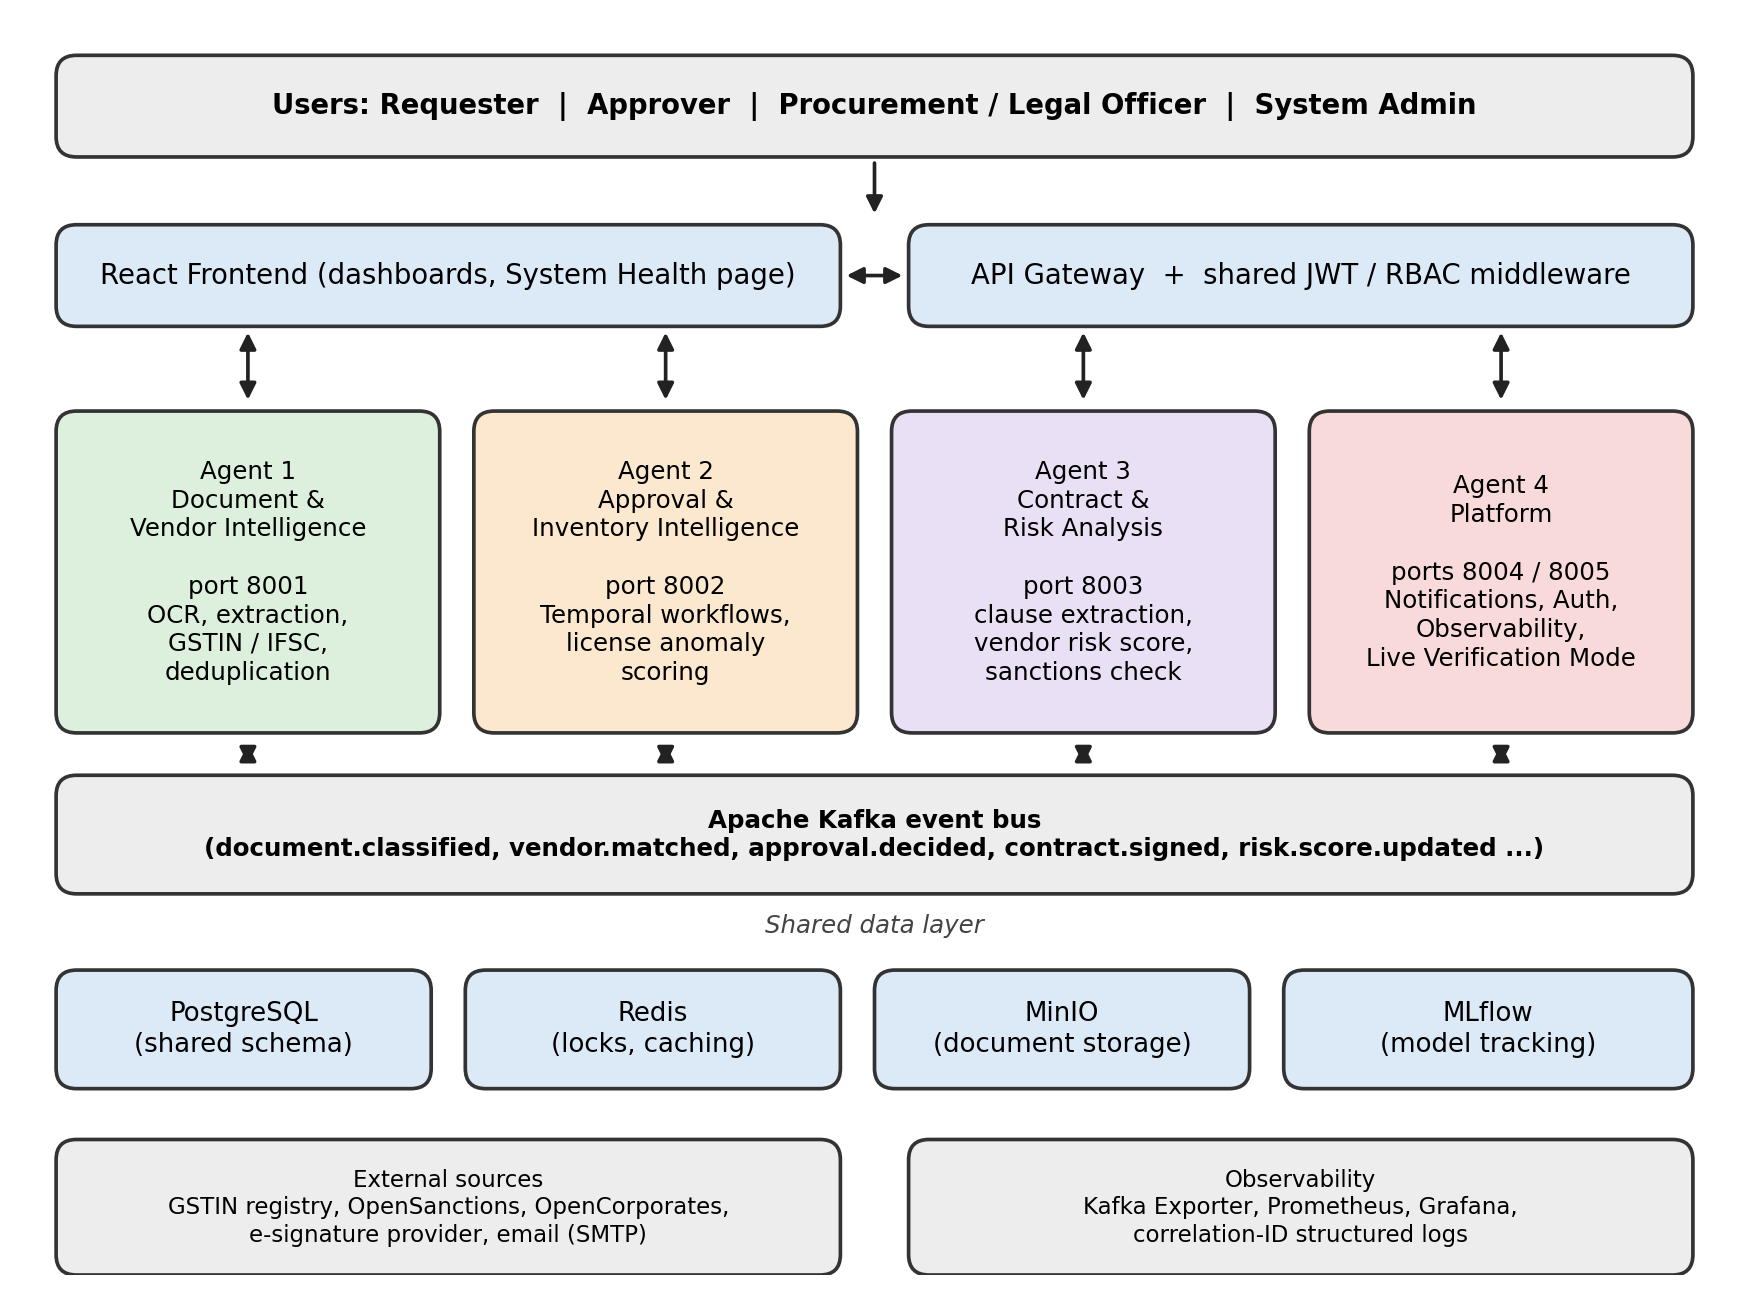
\includegraphics[width=0.92\textwidth]{figures/fig_architecture.png}
\caption{Overall architecture of the proposed system}
\label{fig:arch}
\end{figure}

Splitting the system this way keeps each concern separate. A change to the extraction models does not touch the approval engine, and a slow external lookup cannot block a user's upload, because the heavy work runs asynchronously off the request path.

\subsection{The Four Agents}

Table~\ref{tab:agents} summarises the agents, and the paragraphs that follow describe what each one does.

\begin{table}[!htbp]
\centering
\footnotesize
\renewcommand{\arraystretch}{1.2}
\caption{Summary of the four agents in the proposed system}
\label{tab:agents}
\begin{tabular}{|p{\dimexpr 0.20\textwidth-2\tabcolsep\relax}|p{\dimexpr 0.09\textwidth-2\tabcolsep\relax}|p{\dimexpr 0.35\textwidth-2\tabcolsep\relax}|p{\dimexpr 0.32\textwidth-2\tabcolsep\relax}|}
\hline
\raggedright \textbf{Agent} & \raggedright \textbf{Port} & \raggedright \textbf{Main responsibility} & \raggedright \textbf{Key techniques} \tabularnewline \hline
\raggedright Document and Vendor Intelligence & \raggedright 8001 & \raggedright Document intake, extraction, vendor identity verification, duplicate detection & \raggedright Docling, PaddleOCR, LayoutLMv3 fallback, TF-IDF classifier, rapidfuzz, ClamAV \tabularnewline \hline
\raggedright Approval and Inventory Intelligence & \raggedright 8002 & \raggedright Approval routing, SLA escalation, inventory reservation, license reclaim & \raggedright Temporal, Redis locks, Isolation Forest, SHAP \tabularnewline \hline
\raggedright Contract and Risk Analysis & \raggedright 8003 & \raggedright Contract generation, e-signature, clause extraction, vendor risk scoring, sanctions screening & \raggedright Jinja2, Legal-BERT (CUAD), FinBERT, scikit-learn, PSI drift monitoring \tabularnewline \hline
\raggedright Platform (Notifications, Auth, Observability) & \raggedright 8004 / 8005 & \raggedright Authentication and RBAC, notifications, monitoring, quota control & \raggedright JWT, Kafka consumers, Prometheus, Grafana, Live Verification Mode \tabularnewline \hline
\end{tabular}
\end{table}

\paragraph{Document and Vendor Intelligence.} This agent is the entry point for every document. It scans each upload for malware, extracts structured data, and gives each field a confidence score so that doubtful values go to a human instead of being filled in automatically. It also verifies the vendor's GSTIN and bank details, detects duplicate vendors and duplicate invoices, and never applies a change of payment details directly. Such a change waits in a pending state until a second, different user confirms it.

\paragraph{Approval and Inventory Intelligence.} This agent builds the approval chain for each request from configurable spend and budget rules, excludes the requester from their own chain, and uses Temporal to run SLA timers and escalate automatically when an approver does not respond. It reserves stock and license seats with locks so that two concurrent requests cannot take the last unit. A daily job scores license usage with an Isolation Forest model. When a license looks abandoned, the actual user is told and given seven days to object before it is reclaimed.

\paragraph{Contract and Risk Analysis.} Once a request is approved, this agent fills a contract template, sends it for e-signature and verifies the signing webhook. A question-answering model reads the contract text to pull out the renewal type, notice period and end date, so that reminders can be sent in time. The same agent keeps a running risk score for every vendor from real external sources. Facts such as a sanctions match or a cancelled GSTIN force a High rating, and only the softer signals pass through the learned model.

\paragraph{Platform.} The fourth agent handles what no single functional agent should own: authentication and access control, notification delivery, system monitoring and quota control for scarce external APIs. It also provides the correlation ID that lets one request be followed across all services.

\subsection{Document Processing Pipeline}

The most involved part of the system is the pipeline that turns an uploaded file into a trustworthy structured record, shown in Figure~\ref{fig:pipeline}. The upload returns immediately, and a Kafka consumer runs the stages in the background.

\begin{figure}[!htbp]
\centering
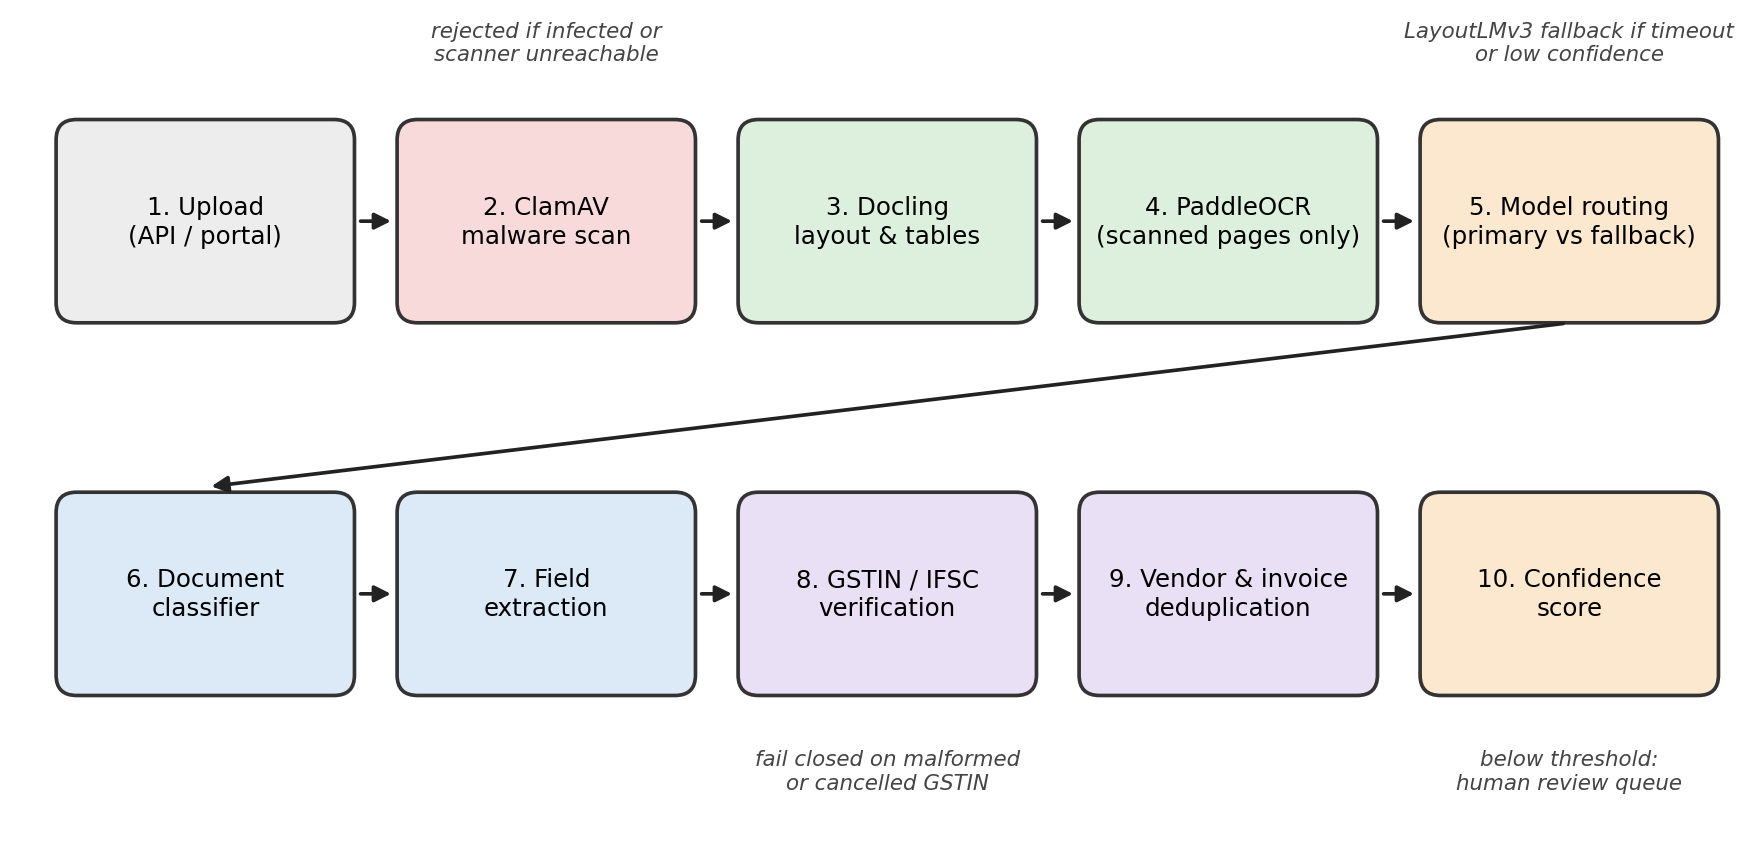
\includegraphics[width=\textwidth]{figures/fig_doc_pipeline.png}
\caption{Document processing pipeline of the Document and Vendor Intelligence agent}
\label{fig:pipeline}
\end{figure}

A file is first streamed through ClamAV and rejected if it is flagged or if the scanner cannot be reached, so the system fails closed. Docling then recovers layout and tables, and PaddleOCR is used only for pages without a text layer. If the primary pipeline times out or its confidence is low, LayoutLMv3 runs as an independent fallback. A trained classifier labels the document as a purchase order, invoice or quote, and the extracted fields are written into the shared schema. The vendor's GSTIN is checked next, and the vendor is matched against existing records, with the GSTIN taking priority over name similarity. Finally, each field receives a confidence score, and anything below the threshold is placed in the review queue.

\subsection{Inter-Agent Communication and Workflow}

Figure~\ref{fig:events} shows how the agents exchange events, and Table~\ref{tab:events} lists the main ones. A single correlation identifier is created at the start of a business flow and carried unchanged through every event and log line, so the full journey of one document or request can be traced.

\begin{figure}[!htbp]
\centering
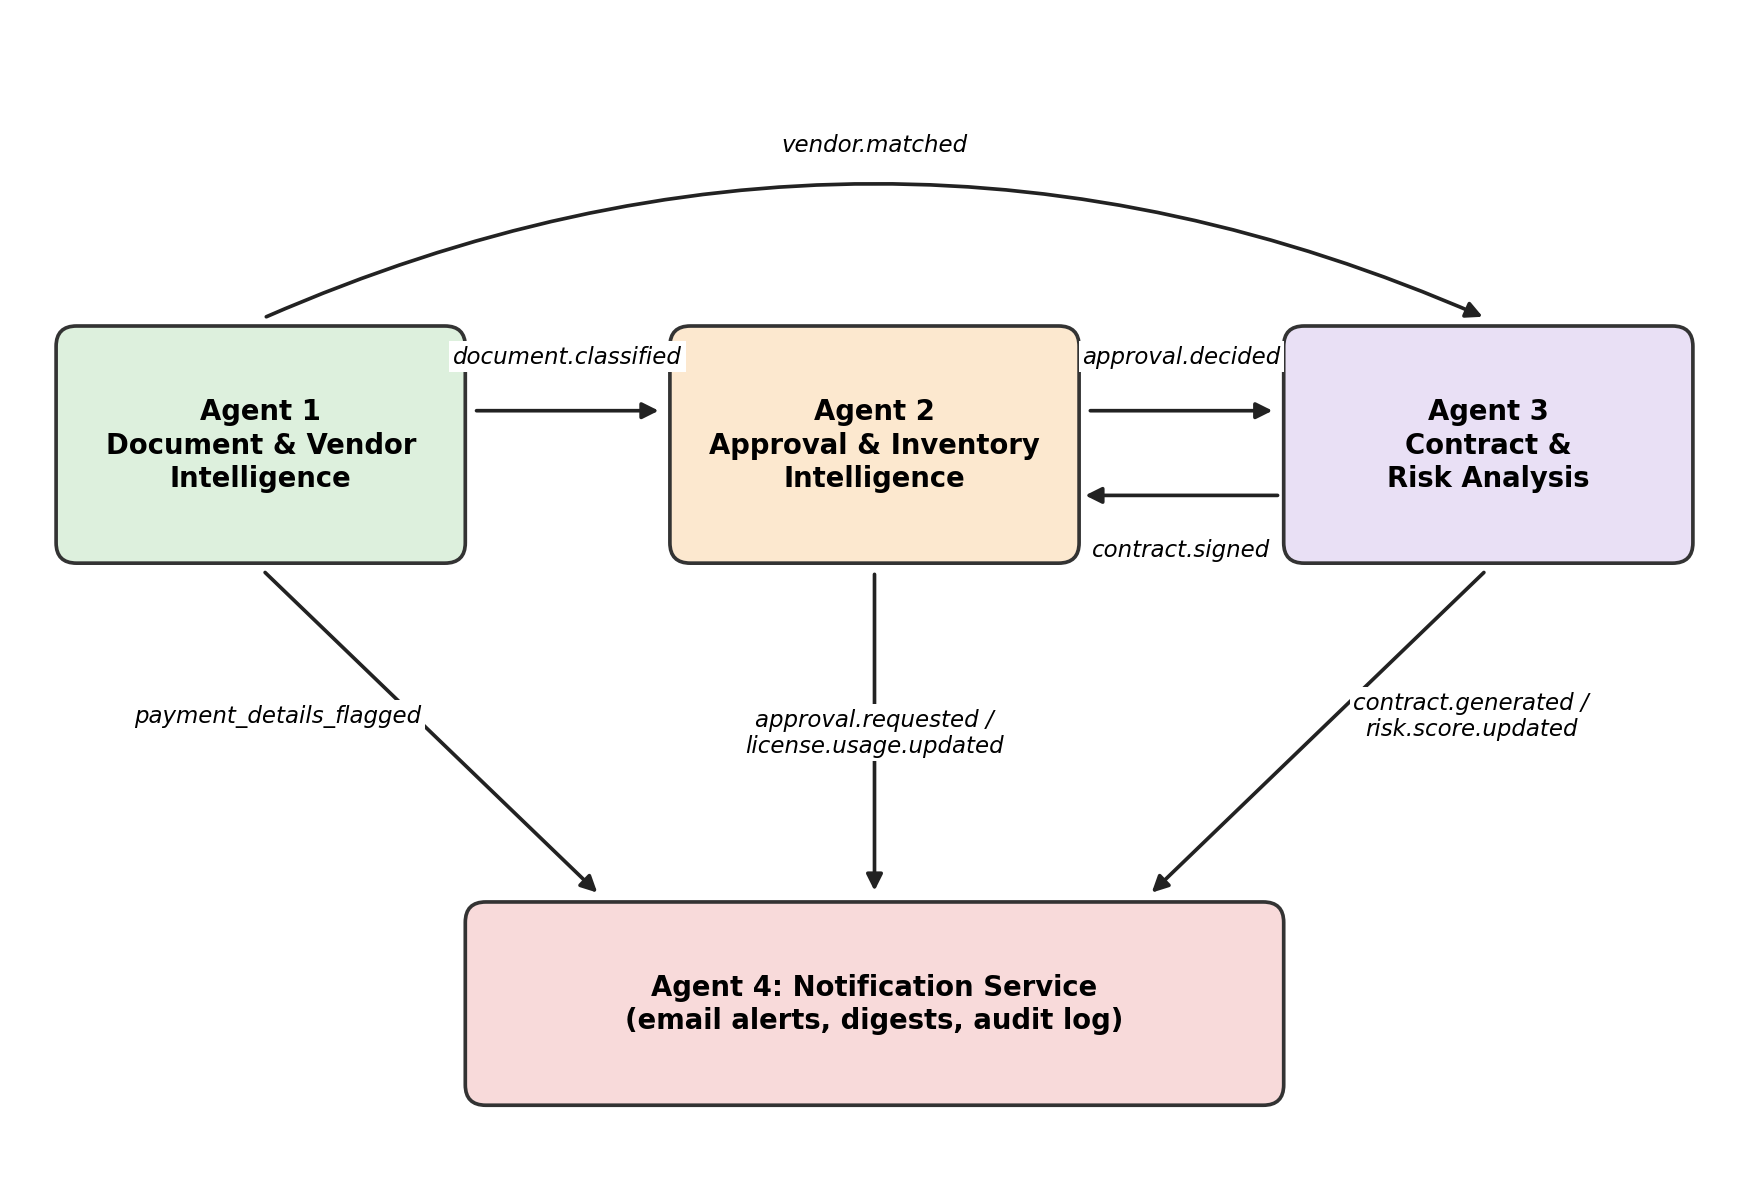
\includegraphics[width=0.9\textwidth]{figures/fig_event_flow.png}
\caption{Event flow between the agents}
\label{fig:events}
\end{figure}

\begin{table}[!htbp]
\centering
\footnotesize
\renewcommand{\arraystretch}{1.2}
\caption{Main events exchanged between agents}
\label{tab:events}
\begin{tabular}{|p{\dimexpr 0.29\textwidth-2\tabcolsep\relax}|p{\dimexpr 0.24\textwidth-2\tabcolsep\relax}|p{\dimexpr 0.43\textwidth-2\tabcolsep\relax}|}
\hline
\raggedright \textbf{Event} & \raggedright \textbf{Published by} & \raggedright \textbf{Consumed by and purpose} \tabularnewline \hline
\raggedright document.classified & \raggedright Agent 1 & \raggedright Agent 2 and notifications: structured extraction result \tabularnewline \hline
\raggedright vendor.matched & \raggedright Agent 1 & \raggedright Agent 3: verified vendor identity for risk scoring \tabularnewline \hline
\raggedright vendor.payment\_\allowbreak details\_\allowbreak flagged & \raggedright Agent 1 & \raggedright Notifications: immediate finance alert on a payment-detail change \tabularnewline \hline
\raggedright approval.requested / approval.decided & \raggedright Agent 2 & \raggedright Agent 3 and notifications: drives contract generation and alerts \tabularnewline \hline
\raggedright license.usage.updated & \raggedright Agent 2 & \raggedright Notifications: utilisation and anomaly alerts \tabularnewline \hline
\raggedright contract.generated / contract.signed & \raggedright Agent 3 & \raggedright Agent 2 and notifications: fulfilment closure \tabularnewline \hline
\raggedright contract.renewal.due & \raggedright Agent 3 & \raggedright Notifications: 60, 30 and 15 day renewal reminders \tabularnewline \hline
\raggedright risk.score.updated & \raggedright Agent 3 & \raggedright Notifications: high-risk alerts \tabularnewline \hline
\end{tabular}
\end{table}

{\sloppy In a typical run, a requester uploads a document and Agent~1 publishes \texttt{document.classified} together with \texttt{vendor.matched}. Agent~2 builds the approval chain and, once the final approver agrees, publishes \texttt{approval.decided}. Agent~3 then generates the contract and sends it for signature, and its \texttt{contract.signed} event tells Agent~2 to mark the request as fulfilled and activate the asset. The notification agent listens to all of these events and sends urgent alerts, such as a flagged payment-detail change, immediately while batching routine ones.\par}

\subsection{Use Case View}

Figure~\ref{fig:usecase} presents the use case diagram of the system. Four actors take part: the System Admin, who configures business rules; the Requester, who submits purchase requests; the Approver, who approves or rejects them; and the Procurement or Legal Officer, who handles vendor documents and contracts. The use cases are grouped into five phases.

\begin{figure}[!htbp]
\centering
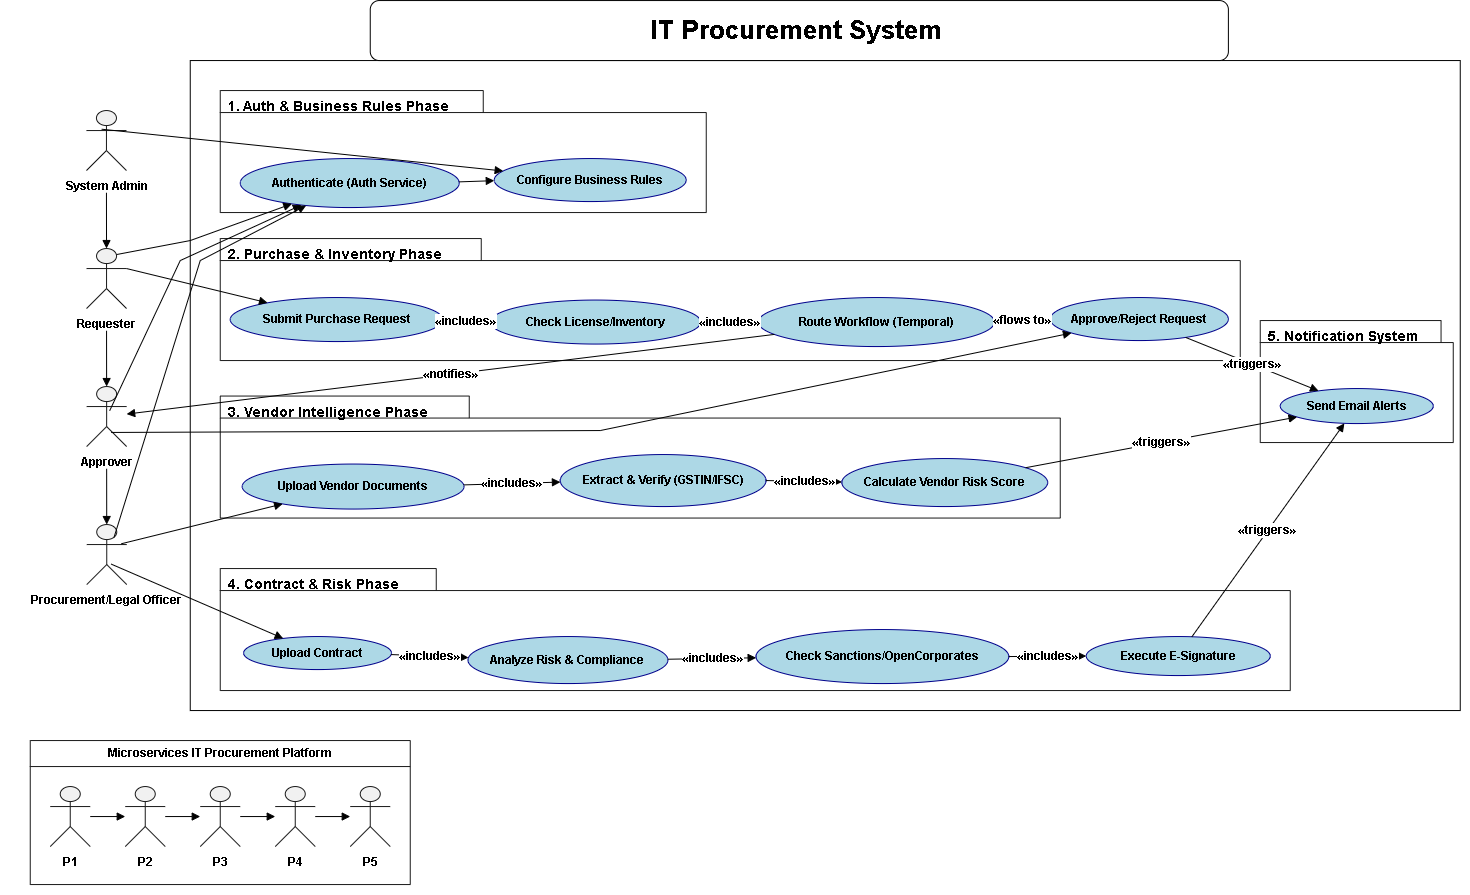
\includegraphics[width=\textwidth]{figures/usecase.png}
\caption{Use case diagram of the IT procurement system}
\label{fig:usecase}
\end{figure}

\begin{enumerate}
\item \textbf{Authentication and business rules.} Users sign in through the authentication service, and the administrator configures the business rules that drive routing.
\item \textbf{Purchase and inventory.} A requester submits a purchase request, the system checks license and inventory availability, the approval workflow is routed through Temporal, and the approver approves or rejects.
\item \textbf{Vendor intelligence.} Vendor documents are uploaded, GSTIN and IFSC details are extracted and verified, and a vendor risk score is calculated.
\item \textbf{Contract and risk.} A contract is uploaded or generated, analysed for risk and compliance, checked against sanctions and company registry data, and finally signed electronically.
\item \textbf{Notification.} Approvals, risk scores and signature events trigger email alerts to the people concerned.
\end{enumerate}

\subsection{Technology Stack}

Table~\ref{tab:stack} lists the main technologies. Wherever possible, pretrained open-source models are used, and only the document classifier and the usage anomaly and risk models are trained within the project.

\begin{table}[!htbp]
\centering
\footnotesize
\renewcommand{\arraystretch}{1.2}
\caption{Technology stack of the proposed system}
\label{tab:stack}
\begin{tabular}{|p{\dimexpr 0.24\textwidth-2\tabcolsep\relax}|p{\dimexpr 0.38\textwidth-2\tabcolsep\relax}|p{\dimexpr 0.34\textwidth-2\tabcolsep\relax}|}
\hline
\raggedright \textbf{Layer} & \raggedright \textbf{Technology} & \raggedright \textbf{Purpose} \tabularnewline \hline
\raggedright Frontend & \raggedright React & \raggedright Dashboards and System Health page \tabularnewline \hline
\raggedright Backend services & \raggedright FastAPI (Python), Docker & \raggedright One containerised service per agent \tabularnewline \hline
\raggedright Messaging & \raggedright Apache Kafka & \raggedright Asynchronous events between agents \tabularnewline \hline
\raggedright Workflow engine & \raggedright Temporal & \raggedright Approval workflows, SLA timers, escalation \tabularnewline \hline
\raggedright Data stores & \raggedright PostgreSQL, Redis, MinIO & \raggedright Records, locks and caching, document files \tabularnewline \hline
\raggedright Document AI & \raggedright Docling, PaddleOCR, LayoutLMv3 & \raggedright Layout analysis, OCR, fallback extraction \tabularnewline \hline
\raggedright Language and risk models & \raggedright Legal-BERT, FinBERT, scikit-learn, SHAP & \raggedright Clause extraction, adverse media, risk and anomaly scoring \tabularnewline \hline
\raggedright Security & \raggedright JWT, ClamAV, Pwned Passwords check & \raggedright Authentication, malware scanning, password safety \tabularnewline \hline
\raggedright Monitoring & \raggedright MLflow, Kafka Exporter, Prometheus, Grafana & \raggedright Model tracking, consumer lag, dashboards \tabularnewline \hline
\raggedright Notifications & \raggedright Jinja2 templates, SMTP (Mailpit in development) & \raggedright Templated email alerts \tabularnewline \hline
\end{tabular}
\end{table}

\subsection{Key Design Principles}

Four principles run through the whole design. The system is \emph{fraud-aware}: uploads are scanned and rejected if the scanner is unavailable, and payment-detail changes need a second person's confirmation. It is \emph{fair}: a user gets a grace period before a license is reclaimed, and a vendor is never scored worse only because some data could not be retrieved. It is \emph{accountable}: every override or sanctions-flag clearance needs a logged justification, and the risk model is monitored for drift. Finally, it is \emph{traceable}: one correlation ID follows a request through every service, and a System Health page shows Kafka lag and recent activity.

%%%%%%%%%%%%%%%%%%%%%%%%%%%%%%%%%%%%%%%%%%%%%%%%%%%
%%% End of Chapter 3
\documentclass[12pt,a4paper]{report}

\usepackage[utf8]{inputenc}
\usepackage[T1]{fontenc}
\usepackage{geometry}
\usepackage{longtable}
\usepackage{array}
\usepackage{booktabs}
\usepackage{ragged2e}
\usepackage{enumitem}
\usepackage{hyperref}

\geometry{
    left=1.25in,
    right=1in,
    top=1in,
    bottom=1in
}

\begin{document}

\chapter{Design of the System}

This chapter describes the requirements, development approach, system
models, resource requirements, and architecture of the Agentic AI-Based
IT Procurement Intelligence Platform. It presents the functional and
non-functional requirements, the principal data flows, the system
layers, and the user-interface design. Diagram positions are identified
where the source report refers to figures that must be inserted or
regenerated.

\section{Requirement Engineering}

Requirement engineering involves identifying the capabilities expected
from the platform, documenting them clearly, and checking that they
remain consistent throughout development. In this project, it was
particularly important because the system is divided into services that
must interoperate through shared event formats, database structures,
REST response conventions, and authentication rules.

\subsection{Requirement Elicitation}

Requirements were identified from the following sources:

\begin{itemize}
    \item \textbf{Review of existing practices and literature:}
    The review in Chapter 2 and the problem analysis in Chapter 3
    identified recurring procurement challenges, including repeated
    manual data entry, unverified vendor details, duplicate invoices,
    delayed approvals, underused software licences, missed contract
    renewals, and infrequent vendor-risk reviews.

    \item \textbf{Stakeholder analysis:}
    The principal users are requesters, approvers and finance users,
    procurement/legal personnel, and system administrators. In the
    implemented demonstration application, the four roles are
    requester, approver, finance, and admin.

    \item \textbf{Guide and team discussions:}
    Discussions were used to prioritise features and distinguish the
    implemented scope from features dependent on external accounts or
    providers. Live GSTIN lookups, sanctions screening, and integration
    with a real e-signature provider may be affected by external
    dependencies or future scope.

    \item \textbf{Review of tools and datasets:}
    Document-processing tools, workflow engines, and relevant datasets
    were reviewed to understand their expected inputs, outputs, and
    practical limitations.
\end{itemize}

The gathered requirements were then grouped into functional and
non-functional requirements.

\subsection{Software Lifecycle Model}

The project followed an iterative and incremental development approach.
This approach was suitable because thresholds, approval rules, model
behaviour, and integration details required testing and refinement
during implementation.

The main practices were:

\begin{itemize}
    \item \textbf{Contract-first design:}
    Shared interfaces were agreed upon before parallel service
    development. These included the Kafka event envelope and topic
    payloads, the base database schema, the REST response envelope,
    and authentication middleware.

    \item \textbf{Service-wise increments:}
    Work was divided across document and vendor, approval and inventory,
    contract and risk, and platform/notification responsibilities.

    \item \textbf{Integration iterations:}
    The services were connected behind a common API gateway.
    Integration testing helped identify issues involving gateway
    routing, Kafka connectivity, and database migrations.

    \item \textbf{Continuous testing:}
    Service-level tests and end-to-end checks were used during
    development rather than postponing all testing until the end.

    \item \textbf{Repeatable deployment:}
    The project uses a \texttt{run.sh} script for bringing up the
    containerised stack, supporting consistent demonstrations and
    verification.
\end{itemize}

\textbf{Figure 4.1:} Iterative and incremental development cycle.
Insert or regenerate the diagram showing contract-first design,
service-wise increments, integration iteration, testing, and
demonstration, with guide feedback informing subsequent iterations.

\subsection{Requirement Analysis}

The requirements are grouped into functional requirements, which
describe what the system should do, and non-functional requirements,
which describe expected qualities and constraints.

\subsubsection{Functional Requirements}

\begin{longtable}{|p{0.8in}|p{3.8in}|p{1.5in}|}
\hline
\textbf{ID} & \textbf{Requirement} & \textbf{Responsible Service} \\
\hline
FR1 & Users can log in and receive access and refresh tokens. Protected
endpoints verify the token and user role, except specified health and
metrics endpoints. & Platform/Authentication \\
\hline
FR2 & Uploaded purchase orders, invoices, and quotations are scanned
for malware before storage. An upload is rejected if the scanner is
unavailable. & Document and Vendor \\
\hline
FR3 & Documents are classified as purchase orders, invoices, or
quotations. Relevant vendor, line-item, total, date, and document-number
fields are extracted. & Document and Vendor \\
\hline
FR4 & Extracted fields receive confidence scores. Results below the
configured threshold, with a default of 0.8, are sent for human review.
& Document and Vendor \\
\hline
FR5 & Vendor records are matched and duplicate documents are detected
using vendor, amount tolerance, and date-window checks.
& Document and Vendor \\
\hline
FR6 & Changes to vendor bank or payment details remain pending until
verified by a different user. & Document and Vendor \\
\hline
FR7 & Purchase requests follow approval routes based on spending tiers,
with service-level-agreement (SLA) timers and escalation.
& Approval and Inventory \\
\hline
FR8 & Approval and rejection decisions are applied through a durable
workflow, and the requester can see the resulting status.
& Approval and Inventory \\
\hline
FR9 & Inventory is reserved using locks to prevent concurrent requests
from reserving the same unit. Oversubscribed requests can be split into
immediate and back-ordered portions. & Approval and Inventory \\
\hline
FR10 & Licence utilisation is calculated, and a reclaim request can be
created when utilisation falls below a configured threshold.
& Approval and Inventory \\
\hline
FR11 & Contracts are generated from templates. Renewal type, notice
period, and end date are extracted, and reminders are scheduled for
60, 30, and 15 days before the notice deadline. & Contract and Risk \\
\hline
FR12 & The system sends contracts for signature and accepts signed-document
callbacks only when the HMAC signature is valid and the callback is not
a replay. & Contract and Risk \\
\hline
FR13 & Vendor risk is represented by a score and band, with contributing
factors listed and urgent alerts raised for a High band.
& Contract and Risk \\
\hline
FR14 & The risk model is monitored for drift; automatic retraining is
not performed. & Contract and Risk \\
\hline
FR15 & Vendor offboarding revokes access, flags active contracts for
review, and sets a data-retention flag rather than deleting records.
& Contract and Risk \\
\hline
FR16 & The notification service consumes events, sends templated email
alerts, prioritises urgent items, supports periodic digests for routine
items, and maintains a searchable notification log. & Notification \\
\hline
FR17 & The frontend provides role-specific navigation and dashboards,
purchase-request submission, approval inbox, document review, vendor,
contract and inventory views, and notification history. & Frontend \\
\hline
\end{longtable}

\subsubsection{Non-Functional Requirements}

\begin{longtable}{|p{1.5in}|p{4.8in}|}
\hline
\textbf{Category} & \textbf{Requirement} \\
\hline
Security & JWT-based authentication and backend role-based access
control; fail-closed malware scanning; HMAC-verified webhooks; and
dual control for payment-detail changes. \\
\hline
Reliability & Approval and renewal workflows are durable. Kafka
consumers are designed for idempotent processing, and webhook replays
are rejected. \\
\hline
Consistency & Endpoints follow a common response envelope, and shared
database changes use idempotent service migrations. \\
\hline
Performance & Uploads return promptly while document extraction and other
heavy processing run asynchronously. \\
\hline
Traceability & A correlation ID follows events and logs. Prometheus
metrics and Grafana dashboards support monitoring of request rate,
latency, errors, and service availability. \\
\hline
Portability & The stack is containerised and intended to run on macOS,
Linux, and Windows through WSL2. \\
\hline
Maintainability & The platform separates responsibilities by service,
uses shared contracts, and includes service-level and end-to-end tests. \\
\hline
Explainability & Risk scores display contributing factors, and
low-confidence extraction results are made available for human review. \\
\hline
\end{longtable}

\textbf{Constraints and assumptions:} Payment execution, ERP
integration, tax identifiers other than GSTIN and IFSC, and automatic
model retraining are outside the stated scope. Parts of the training
data are synthetic, and the availability of live external lookups
depends on free-tier quotas and external services.

\subsection{UML Diagrams and Data Flow Diagrams}

The diagrams in this section should be numbered consistently and
referenced in the text. Insert the actual diagrams as images or
recreate them in the final document.

\subsubsection{Use Case Diagram}

The use case diagram is presented in Figure 3.4 in Chapter 3. It
identifies the System Admin, Requester, Approver, and Procurement/Legal
Officer and groups the main activities into authentication and business
rules, purchase and inventory, vendor intelligence, contract and risk,
and notifications.

\subsubsection{Data Flow Diagram -- Level 0}

The Level 0 context diagram should represent the platform as one
process and show its interactions with the external entities identified
in the project. Insert the Level 0 diagram here and ensure its external
entities and labelled data flows are legible.

\subsubsection{Data Flow Diagram -- Level 1}

The Level 1 diagram decomposes the platform into the processes listed
in Table 4.2. Processes 2.0--6.0 exchange events through the
Kafka-compatible messaging layer; they should not be shown as direct
synchronous calls unless such a call is implemented.

\begin{longtable}{|p{0.65in}|p{1.4in}|p{2in}|p{2.3in}|}
\hline
\textbf{Process} & \textbf{Name} & \textbf{Inputs} & \textbf{Outputs} \\
\hline
1.0 & Authenticate & Login credentials or refresh token &
Access/refresh tokens and user role \\
\hline
2.0 & Ingest and extract documents & Uploaded file and request details &
Classified/extracted document, vendor match, review-queue items \\
\hline
3.0 & Approve and reserve & Purchase request and approval/rejection
signal & Decision, stock/licence reservations, escalations \\
\hline
4.0 & Manage contracts & Approved request and signed callback &
Generated contract, signature status, renewal reminders \\
\hline
5.0 & Score vendor risk & Vendor data and outcomes &
Risk score, band, contributing factors, drift flag \\
\hline
6.0 & Notify & Events from processes 2.0--5.0 &
Emails, digests, notification log \\
\hline
\end{longtable}

\subsubsection{Sequence Diagram}

The sequence diagram should show the purchase-request journey from the
requester and frontend/gateway through document intake, Kafka, the
approval API and worker, Temporal, the contract service, and the
notification service, ending with the signed-contract event and
request-status update.

\subsubsection{Activity Diagram: Document Processing}

The document-processing activity flow begins with upload and malware
scanning. The upload is rejected if the file is flagged or the scanner
is unavailable. A clean file proceeds through parsing, classification,
field extraction, vendor matching, duplicate checking, and confidence
scoring. Results meeting the threshold can be completed; lower-confidence
results are sent to a human review queue.

\textbf{Figure 4.2:} Activity diagram of document processing. Insert
the regenerated diagram with readable decision branches and labels.

\subsubsection{Class/Entity Relationship Diagram}

The principal entities identified in the report are User, Vendor,
PurchaseRequest, Document, ExtractedField, ApprovalRecord,
InventoryItem, LicenseUsage, Contract, RiskScore, Notification, and
RenewalReminder. The diagram should show the relationships described in
the project: a requester raises purchase requests; requests refer to
vendors and can have documents and approval records; vendors can have
documents, contracts, and risk scores; documents have extracted fields;
contracts have renewal reminders; and inventory items are associated
with licence-usage records.

The exact table definitions are maintained in the shared database
schema and service migrations.

\textbf{Figure 4.3:} Entity relationship diagram. Insert the regenerated
diagram and check that cardinalities and relationship labels are
readable and consistent with the actual database schema.

\subsection{Cost Analysis}

The project uses open-source software, so the report identifies no
additional software-licence cost. Development is based on existing
student laptops. The principal potential costs are team effort, external
API usage beyond free tiers, optional cloud hosting, and a production
email/domain service. The estimates below are indicative and should be
updated if actual quotations or usage figures become available.

\begin{longtable}{|p{1.5in}|p{3.5in}|p{1.4in}|}
\hline
\textbf{Item} & \textbf{Basis} & \textbf{Indicative Cost} \\
\hline
Software licences & Python, FastAPI, PostgreSQL, Redis, Redpanda/Kafka,
MinIO, Temporal, MLflow, Prometheus, Grafana, ClamAV, Docling, React,
Docker and other listed open-source tools & Rs. 0 \\
\hline
Development hardware & Existing student laptops & Rs. 0 additional \\
\hline
External APIs & Free tiers where available; usage depends on provider
limits & Depends on usage \\
\hline
Team effort & Part-time project work by team members & Not monetised \\
\hline
Optional cloud hosting & Pilot virtual machine with approximately
8 vCPU and 16 GB RAM, plus storage and backups &
Approx. Rs. 6,000--10,000 per month \\
\hline
Domain and email delivery & Production SMTP service in place of
development mail tooling & A few hundred rupees per month at pilot
volume \\
\hline
\end{longtable}

A meaningful break-even estimate requires measured monthly document
volume, average licence costs, and an estimate of time saved or duplicate
payments avoided. Those figures are not specified here, so no
return-on-investment claim is made.

\subsection{Hardware and Software Requirements}

The stack runs multiple containers concurrently. The document parser
and ClamAV can be resource-intensive; therefore, the recommended
configuration is expected to provide a smoother development and
demonstration experience.

\begin{longtable}{|p{1.5in}|p{2in}|p{2.5in}|}
\hline
\textbf{Component} & \textbf{Minimum} & \textbf{Recommended} \\
\hline
Processor & 4 cores & 8 cores \\
\hline
Memory & 8 GB RAM & 16 GB RAM \\
\hline
Storage & 25 GB free & 50 GB free for images, model files, and
database volumes \\
\hline
Network & Required for initial builds, image pulls, and ClamAV
definition updates & Broadband connection \\
\hline
GPU & Not required & Optional for heavier OCR or transformer workloads \\
\hline
\end{longtable}

\begin{longtable}{|p{1.7in}|p{4.3in}|}
\hline
\textbf{Category} & \textbf{Requirement} \\
\hline
Operating system & macOS, Ubuntu/Linux, or Windows 10/11 with WSL2 \\
\hline
Container runtime & Docker Engine or Docker Desktop with Docker Compose \\
\hline
Backend & Python with FastAPI, SQLAlchemy, Alembic, pytest,
scikit-learn, rapidfuzz, and Jinja2 \\
\hline
Frontend & React, TypeScript, Vite, and Tailwind CSS; the frontend is
built in a Node 20 container \\
\hline
Data and messaging & PostgreSQL, Redis, Redpanda (Kafka API), and MinIO \\
\hline
Workflow and ML & Temporal and MLflow \\
\hline
Document processing & Docling, pdfplumber, Tesseract OCR, and ClamAV \\
\hline
Monitoring and mail & Prometheus, Grafana, and Mailpit \\
\hline
Gateway & Nginx \\
\hline
Browser & A current version of Chrome, Edge, Firefox, or Safari \\
\hline
\end{longtable}
\section{System Architecture}

The Agentic AI-Based IT Procurement Intelligence Platform follows a
modular, event-driven architecture. The system is divided into
independent services, each responsible for a specific procurement
function. This separation improves maintainability, supports parallel
development, and allows background tasks to be processed independently
of user-facing requests.

The frontend communicates with backend services through a common API
gateway. Synchronous HTTP requests are used for operations that require
an immediate response, while inter-service communication primarily
uses a Kafka-compatible messaging layer. Temporal supports durable
workflows such as approvals, escalations, and contract-renewal
processes.

PostgreSQL stores application records, Redis supports caching and
locking, and MinIO stores uploaded documents. Background workers
process events and execute tasks that may take longer to complete.
This design allows the application to return responses to users
without waiting for every downstream operation to finish.

\subsection{UI/UX Design}

The frontend is implemented as a React and TypeScript single-page
application using Vite and Tailwind CSS. Nginx serves the frontend
and routes API requests to the appropriate backend services. Serving
the frontend and API through a common entry point simplifies access
to the application.

The interface is designed around the responsibilities of the four
implemented roles: requester, approver, finance, and administrator.

The following design principles guide the user interface:

\begin{enumerate}[label=\arabic*.]
    \item \textbf{Role-aware navigation:}
    The interface provides navigation appropriate to requesters,
    approvers, finance users, and administrators. Frontend route
    checks improve usability but do not replace backend
    authorization.

    \item \textbf{Clear asynchronous status:}
    The interface communicates the status of document classification,
    extraction, approvals, and other operations that may take time
    to complete.

    \item \textbf{Transparent system limitations:}
    The interface should distinguish successful operations from
    pending or failed operations. It should not indicate that an
    action succeeded when the backend is unavailable.

    \item \textbf{Human review:}
    Users can review extracted document fields and their confidence
    scores. Where correction is supported, users can correct the
    extracted information before proceeding.

    \item \textbf{Demonstration support:}
    The login interface supports demonstration through demo-role
    switching, allowing the different role-specific workflows to
    be presented during project evaluation.
\end{enumerate}

The principal screens and their purposes are summarised in
Table 4.3.

\begin{longtable}{|p{1.35in}|p{1.35in}|p{3in}|}
\hline
\textbf{Screen} & \textbf{User Role} & \textbf{Purpose} \\
\hline
Login & All roles & Sign in or select a demonstration role. \\
\hline
Requester Dashboard & Requester & View submitted purchase requests and their current status. \\
\hline
New Request Wizard & Requester & Enter request details, select a vendor, optionally upload a document, review extracted fields, and submit the request. \\
\hline
Approval Inbox & Approver, Finance & Review pending requests and approve or reject them according to assigned permissions. \\
\hline
Document Review & Approver, Finance, Admin & Review extracted document fields and confidence scores, and correct and save fields where supported. \\
\hline
Vendor Profile & Finance, Admin & View vendor risk information and the payment-change verification queue, along with supported vendor actions. \\
\hline
Contracts & Admin & Generate contracts, manage the signature workflow, and view contract-renewal timelines. \\
\hline
Inventory & Approver, Admin & View hardware stock and software-licence utilisation. \\
\hline
Notification Log & All, subject to permissions & View sent, queued, and failed notifications. \\
\hline
Global Search & All, subject to permissions & Search available purchase requests, vendors, contracts, and documents. \\
\hline
\end{longtable}

\textbf{Figure 4.4: Main-screen wireframes of the platform.}

Insert screenshots or labelled wireframes of the login screen,
new-request wizard, approval inbox, and vendor profile. Replace
this instruction with the actual figure before submitting the
final report.

\subsection{Block Diagram}

The block diagram represents the major components of the platform
and the relationships between them. It should show the frontend,
gateway, application services, background workers, messaging and
workflow components, data stores, and monitoring tools.

The main architectural layers are described in Table 4.4.

\begin{longtable}{|p{1.4in}|p{4.3in}|}
\hline
\textbf{Layer} & \textbf{Components and Responsibilities} \\
\hline
Clients & The browser-based React application and API clients access the platform through the API gateway on port 8080. \\
\hline
Gateway & Nginx serves the frontend and routes API paths to the appropriate backend services, providing a common entry point. \\
\hline
Application Services & The Document and Vendor Agent runs on port 8001; the Approval and Inventory Agent on port 8002; the Contract and Risk Agent on port 8003; the Notification Agent on port 8004; and the Authentication Service on port 8005. Authentication and role-based middleware protect application endpoints, except for specifically designated health and metrics endpoints. \\
\hline
Background Workers & Each domain service can use a background worker to consume events and perform asynchronous processing and workflow-related tasks. \\
\hline
Messaging and Orchestration & Redpanda provides a Kafka-compatible event-messaging interface. Temporal supports durable workflows for approvals, escalations, and contract renewals. \\
\hline
Data and Platform Services & PostgreSQL stores application records, Redis supports caching and locks, and MinIO stores documents. ClamAV scans files for malware, MLflow supports model tracking, and Mailpit supports development email testing. \\
\hline
Observability & Prometheus collects metrics and Grafana provides dashboards for monitoring request rates, latency, errors, and service availability. \\
\hline
\end{longtable}

\textbf{Figure 4.5: Block diagram of the proposed system architecture.}

Insert a clean block diagram based on the architecture described
above. Verify that the service names, ports, gateway routes,
workers, event bus, workflow engine, data stores, and monitoring
components correspond to the implemented system.

\subsection{Main Data Paths}

The principal data paths in the system are described below.

\begin{enumerate}[label=\arabic*.]
    \item \textbf{User access:}
    The browser accesses the frontend through Nginx. API requests
    are routed to the appropriate backend service.

    \item \textbf{Document processing:}
    The Document and Vendor Agent scans an uploaded file for
    malware. Accepted files are stored in MinIO, and an ingestion
    event is published. Background processing extracts and
    classifies document information and publishes the resulting
    classification and vendor-matching information.

    \item \textbf{Approval processing:}
    The Approval and Inventory Agent interacts with the workflow
    engine to initiate or progress approval workflows. Background
    workers execute workflow-related tasks, apply decisions, and
    publish relevant events.

    \item \textbf{Contract processing:}
    The Contract and Risk Agent processes approved requests,
    generates contracts, and handles signed-document callbacks.
    The callback is accepted only after the required HMAC
    signature validation and replay checks. A contract-signed
    event is published, allowing the Approval and Inventory
    Agent to update the purchase-request status.

    \item \textbf{Risk assessment and notifications:}
    The Contract and Risk Agent publishes relevant risk-score
    and renewal events. The Notification Agent consumes
    applicable events and sends email notifications through
    the configured SMTP service.

    \item \textbf{Data access and supporting services:}
    Application services use PostgreSQL for persistent records.
    Redis supports approval and contract locking, MinIO stores
    documents, and MLflow supports tracking of contract and
    risk-model experiments.
\end{enumerate}

These data paths illustrate how synchronous API operations,
event-driven communication, and durable workflows work together
to support procurement activities.

\section{Chapter 4 Review Checklist Before Submission}

Before submitting this chapter for final review, verify the following
items:

\begin{enumerate}[label=\arabic*.]
    \item Replace every instruction to insert a diagram, wireframe,
    or screenshot with the actual figure, or remove the placeholder
    if the figure is not included in the final scope.

    \item Ensure that figure numbers and table numbers are unique
    and sequential throughout the report. Check consistency with
    the numbering used in Chapter 3.

    \item Verify service names, ports, user roles, event names,
    software versions, and system behaviour against the actual
    implementation.

    \item Recheck the cost estimates and any statements about
    external services, free-tier limits, and third-party
    integrations. Clearly identify estimates that have not been
    confirmed through actual quotations or usage data.

    \item Confirm that the functional and non-functional
    requirements describe implemented features accurately and
    distinguish implemented functionality from planned or
    externally dependent features.

    \item Update the table of contents, list of figures, and
    list of tables after integrating the chapter into the
    complete report.
\end{enumerate}

\end{document}


\chapter{Result and Discussion} \label{chap5}
\newpage

\section{Screenshots of the System}

\section{Sample Code (of imp part/ main logic)}

\section{Testing}
\subsection{Unit Testing}
\subsection{Integration Testing}
\subsection{Blackbox Testing}
% Chapter 10 Conclusion

\chapter{Conclusion \& Future Scope} \label{chap6}
\newpage

In this report, the study of different domain techniques is presented. The different techniques such as ABC, XYZ, content-based, and collaborative filtering are explained with examples. The different hybrid approaches are also described. The comparative study of various techniques mentioned above is presented in this report. The hybrid approach is proposed with xyz modification. The performance measures like precision and recall are described in this report. The different standard datasets or variable inputs are defined that may be used in experiments for this domain system. The two datasets identified for experiments are CDEF and JKLM. The applications of this domain are identified and presented. 



% End of Chapter

\addcontentsline{toc}{chapter}{References}

\begin{thebibliography}{11}

\bibitem{xu2020layoutlm}
Y.~Xu, M.~Li, L.~Cui, S.~Huang, F.~Wei, and M.~Zhou, ``LayoutLM: Pre-training of text and layout for document image understanding,'' in \emph{Proc. ACM SIGKDD}, 2020.

\bibitem{huang2022layoutlmv3}
Y.~Huang, T.~Lv, L.~Cui, Y.~Lu, and F.~Wei, ``LayoutLMv3: Pre-training for document AI with unified text and image masking,'' in \emph{Proc. ACM Multimedia}, 2022.

\bibitem{auer2024docling}
C.~Auer \emph{et al.}, ``Docling technical report,'' arXiv:2408.09869, 2024.

\bibitem{cui2025paddleocr}
C.~Cui \emph{et al.}, ``PaddleOCR 3.0 technical report,'' arXiv:2507.05595, 2025.

\bibitem{hendrycks2021cuad}
D.~Hendrycks, C.~Burns, A.~Chen, and S.~Ball, ``CUAD: An expert-annotated NLP dataset for legal contract review,'' in \emph{NeurIPS Datasets and Benchmarks}, 2021.

\bibitem{chalkidis2020legalbert}
I.~Chalkidis \emph{et al.}, ``LEGAL-BERT: The muppets straight out of law school,'' in \emph{Findings of EMNLP}, 2020.

\bibitem{araci2019finbert}
D.~Araci, ``FinBERT: Financial sentiment analysis with pre-trained language models,'' arXiv:1908.10063, 2019.

\bibitem{liu2008isolation}
F.~T. Liu, K.~M. Ting, and Z.-H. Zhou, ``Isolation forest,'' in \emph{Proc. IEEE ICDM}, 2008.

\bibitem{lundberg2017shap}
S.~M. Lundberg and S.-I. Lee, ``A unified approach to interpreting model predictions,'' in \emph{Proc. NeurIPS}, 2017.

\bibitem{wu2023autogen}
Q.~Wu \emph{et al.}, ``AutoGen: Enabling next-gen LLM applications via multi-agent conversation,'' arXiv:2308.08155, 2023.

\bibitem{kreps2011kafka}
J.~Kreps, N.~Narkhede, and J.~Rao, ``Kafka: A distributed messaging system for log processing,'' in \emph{Proc. NetDB Workshop}, 2011.

\end{thebibliography}


% Acknowledgement
\addcontentsline{toc}{chapter}{Acknowledgement}
% Acknowledgment Page

\begin{centering}
    \large
{\LARGE\bf Acknowledgement}\\
\end{centering}
    
\justify
The success of a project like this, involving high technical expertise, patience, and massive support from guides, is possible when team members work together. We take this opportunity to express our gratitude to those who have been instrumental in the successful completion of this project. We would like to show our appreciation to \textbf{Prof. Guide Name} for their tremendous support and help; without them, this project would not have reached fruition. We would also like to thank our project coordinator \textbf{Dr. Rakhi Kalantri} for providing us with regular inputs about documentation and project timeline. A big thanks to our HOD \textbf{Dr. M.Kiruthika } for all the encouragement given to our team. We would also like to thank our principal, \textbf{Dr. S. M. Khot}, and our college, \textbf{Fr. C. Rodrigues Institute of Technology, Vashi}, for giving us the opportunity and the environment to learn and grow.

\vspace{3cm}
\hfill% move it to the right
\begin{tabular}[t]{l@{}}
\vspace{1cm}

{\textbf{Project Group Members:}} \\ 
\vspace{1cm}

1. Student 1 Name, Roll No \\
\noindent\rule{5cm}{0.10pt} \\
\\
\vspace{1cm}

2. Student 2 Name, Roll No \\
\noindent\rule{5cm}{0.10pt} \\
\\
\vspace{1cm}

3. Student 3 Name, Roll No \\
 \noindent\rule{5cm}{0.10pt}
\\
\vspace{1cm}
\end{tabular}

%%%%%%%%%%%%%%%%%%%%%%%%%%%%%%%%%%%%
%\begin{flushright} 
%\vspace{0.5in}
%\noindent\rule{4cm}{0.4pt} \\ (Signature)\\
%\vspace{0.3in}
%\noindent\rule{4cm}{0.4pt} \\ (Name of the Student)
%\end{flushright}
%\vspace{0.5cm}
%{\bf Date:} \\
%%%%%%%%%%%%%%%%%%%%%%%%%%%%%%%%%%%%
%% End of Acknowledgement Page


% Appendix A: Timeline Chart
\addcontentsline{toc}{chapter}{Appendix A: Timeline Chart}
% Fun Fact :- Only way to add vertical spacing in lateX is to use \vspace* coz \vspace is deleted if it is at the beginning. Use it wisely

\vspace*{5cm}
\begin{centering}
    \large
{\LARGE\bf Appendix A : Timeline Chart}\\
\end{centering}

\newpage

This is appendix A

% Appendix B: Sustainable Development Goal (SDG) Mapping
\addcontentsline{toc}{chapter}{Appendix B: Sustainable Development Goal (SDG) Mapping}
\chapter*{Appendix B}

\label{app:sdg_mapping}

The project team has identified the following Sustainable Development Goal(s) (SDG) relevant to the proposed project. The mapping should demonstrate a clear and meaningful relationship between the project problem, proposed solution, and the selected SDG(s).

\vspace{0.4cm}

\begin{center}
\textbf{\large SDG Mapping of the Project}
\end{center}

\vspace{0.3cm}

%------------------------------------------------
% SDG Mapping Table
%------------------------------------------------

\renewcommand{\arraystretch}{1.4}

\begin{center}
\begin{tabular}{|c|c|p{4.2cm}|p{6.0cm}|}
\hline
\textbf{Sr. No.} &
\textbf{SDG No.} &
\textbf{Complete Name of SDG} &
\textbf{Rationale / Contribution of the Project} \\
\hline

1 &
\_\_\_\_ &
\parbox[t]{4.2cm}{
\vspace{0.15cm}
\_\_\_\_\_\_\_\_\_\_\_\_\_\_\_\_\_\_\_\_
\vspace{1.4cm}
} &
\parbox[t]{6.0cm}{
\vspace{0.15cm}
Explain how the project contributes to this
SDG and the specific problem addressed.
\vspace{1.4cm}
}
\\
\hline

2 &
\_\_\_\_ &
\parbox[t]{4.2cm}{
\vspace{0.15cm}
\_\_\_\_\_\_\_\_\_\_\_\_\_\_\_\_\_\_\_\_
\vspace{1.4cm}
} &
\parbox[t]{6.0cm}{
\vspace{0.15cm}
Explain how the project contributes to this
SDG and the specific problem addressed.
\vspace{1.4cm}
}
\\
\hline

3 &
\_\_\_\_ &
\parbox[t]{4.2cm}{
\vspace{0.15cm}
\_\_\_\_\_\_\_\_\_\_\_\_\_\_\_\_\_\_\_\_
\vspace{1.4cm}
} &
\parbox[t]{6.0cm}{
\vspace{0.15cm}
Explain how the project contributes to this
SDG and the specific problem addressed.
\vspace{1.4cm}
}
\\
\hline

\end{tabular}
\end{center}

\vspace{0.5cm}

%------------------------------------------------
% Guidelines
%------------------------------------------------

\noindent
\textbf{Guidelines for Students:}

\begin{itemize}
    \item Identify only the SDG(s) that have a direct and meaningful
    connection with the project.
    
    \item Mention the \textbf{official SDG number and complete name}.
    
    \item Provide a clear rationale explaining how the project
    contributes to the selected SDG.
    
    \item Avoid mapping an SDG merely because the project falls within
    a particular technology domain.
    
    \item The SDG mapping should be discussed and validated with the
    Project Guide.
\end{itemize}

\vspace{1.0cm}

%------------------------------------------------
% Guide Verification
%------------------------------------------------

\begin{center}

\rule{6cm}{0.2px}\\
\textbf{Signature of Project Guide}\\[0.4cm]

Name of Project Guide: \rule{5cm}{0.2px}\\[0.4cm]

Date: \rule{3cm}{0.2px}

\end{center}



% Appendix C: Complex Engineering Problem Identification and Evaluation
\addcontentsline{toc}{chapter}{Appendix C: Complex Engineering Problem Identification and Evaluation}
%=========================================================
% APPENDIX C
% COMPLEX ENGINEERING PROBLEM IDENTIFICATION AND EVALUATION
%=========================================================

\chapter*{Appendix C}

{Appendix C: Complex Engineering Problem Identification and Evaluation}

\begin{center}
    {\Large\bfseries COMPLEX ENGINEERING PROBLEM}\\[0.15cm]
    {\Large\bfseries IDENTIFICATION AND EVALUATION}
\end{center}

\vspace{0.3cm}

\noindent
The Washington Accord emphasizes the ability of engineering graduates
to identify, analyse and solve complex engineering problems using
appropriate engineering knowledge, modern tools, multidisciplinary
thinking and analytical reasoning. The Major Project provides an
opportunity for students to demonstrate these abilities through a
structured and evidence-based project.

\vspace{0.25cm}

\noindent
This appendix provides a structured mechanism to assess the complexity
of the proposed Major Project. The assessment is initially carried out
by the student team and subsequently verified by the Project Guide.

%---------------------------------------------------------
% A. PROJECT DETAILS
%---------------------------------------------------------

\section*{A. Project Details}

\begin{center}
\renewcommand{\arraystretch}{1.4}

\begin{tabular}{|p{5cm}|p{9cm}|}
\hline
\textbf{Project Title} & \\[0.5cm]
\hline
\textbf{Group / Team No.} & \\[0.4cm]
\hline
\textbf{Name of Student(s)} & \\[0.7cm]
\hline
\textbf{Project Guide} & \\[0.4cm]
\hline
\textbf{Academic Year} & \\[0.4cm]
\hline
\end{tabular}

\end{center}

%---------------------------------------------------------
% B. COMPLEXITY EVALUATION
%---------------------------------------------------------

\section*{B. Complexity Evaluation}

\noindent
For each parameter, the student team shall assign a score from
\textbf{0 to 3} and provide a suitable justification or evidence.
The Project Guide shall review the student's assessment and record
the verified score in the final column.

\vspace{0.3cm}

\begin{center}

\small
\renewcommand{\arraystretch}{1.35}

\begin{tabularx}{\textwidth}{|
>{\centering\arraybackslash}p{0.7cm}|
p{3.8cm}|
>{\centering\arraybackslash}p{1.1cm}|
X|
>{\centering\arraybackslash}p{1.1cm}|}

\hline

\textbf{Sr. No.} &
\textbf{Complexity Parameter} &
\textbf{Student Score} &
\textbf{Student Justification / Evidence} &
\textbf{Guide Score} \\

\hline

1 &
Problem novelty and research depth &
&
&
\\[0.8cm]

\hline

2 &
Multidisciplinary knowledge requirement &
&
&
\\[0.8cm]

\hline

3 &
System design complexity &
&
&
\\[0.8cm]

\hline

4 &
Technology integration &
&
&
\\[0.8cm]

\hline

5 &
Data analysis and experimentation &
&
&
\\[0.8cm]

\hline

6 &
Societal / industrial relevance &
&
&
\\[0.8cm]

\hline

7 &
Stakeholder involvement &
&
&
\\[0.8cm]

\hline

8 &
Sustainability considerations &
&
&
\\[0.8cm]

\hline

\multicolumn{2}{|r|}{\textbf{Total Score}} &
\textbf{/24} &
&
\textbf{/24} \\

\hline

\end{tabularx}

\end{center}

%---------------------------------------------------------
% SCORING GUIDELINE
%---------------------------------------------------------

\vspace{0.3cm}

\noindent
\textbf{Scoring Guideline}

\vspace{0.1cm}

\begin{center}

\renewcommand{\arraystretch}{1.25}

\begin{tabular}{|c|p{8.5cm}|}
\hline
\textbf{Score} & \textbf{Interpretation} \\
\hline
0 & Not applicable / negligible \\
\hline
1 & Basic level of complexity \\
\hline
2 & Moderate level of complexity \\
\hline
3 & Significant / high level of complexity \\
\hline
\end{tabular}

\end{center}

\vspace{0.3cm}

\noindent
\textbf{Maximum Score: 24}

%---------------------------------------------------------
% C. FINAL PROJECT CLASSIFICATION
%---------------------------------------------------------

\section*{C. Final Project Classification}

\noindent
The final classification shall be based on the score verified by the
Project Guide.

\vspace{0.25cm}

\begin{center}

\renewcommand{\arraystretch}{1.4}

\begin{tabular}{|c|p{6.5cm}|}
\hline
\textbf{Score Range} & \textbf{Project Classification} \\
\hline
0--8 & Simple Engineering Problem \\
\hline
9--16 & Moderately Complex Engineering Problem \\
\hline
17--24 & Complex Engineering Problem \\
\hline
\end{tabular}

\end{center}

\vspace{0.35cm}

\noindent
\textbf{Final Classification:}

\vspace{0.15cm}

\noindent
$\square$ Simple Engineering Problem

\vspace{0.15cm}

\noindent
$\square$ Moderately Complex Engineering Problem

\vspace{0.15cm}

\noindent
$\square$ Complex Engineering Problem

%---------------------------------------------------------
% D. GUIDE'S FINAL REMARKS
%---------------------------------------------------------


\centering
\textbf{Project Guide Signature}
\\[0.8cm]

\centering
Date: \rule{3cm}{0.4pt}



%=========================================================
% END OF APPENDIX C
%=========================================================

% Appendix D: Project Outcomes
\addcontentsline{toc}{chapter}{Appendix D: Project Outcomes}
% Appendix D: Project Outcomes

\vspace*{5cm}
\begin{centering}
{\LARGE\bfseries Appendix D: Project Outcomes}\\
\end{centering}

\newpage

\section*{Publications and Competitions}
\begin{center}
\tablestyle
\begin{tabularx}{\textwidth}{|L{0.22\textwidth}|Y|L{0.18\textwidth}|}
\hline
\textbf{Outcome} & \textbf{Details} & \textbf{Status} \\ \hline
Research paper & A paper on calibrated, evidence-based review gates for procurement documents (provisional title: \emph{Agentic AI Procurement Solution}) & Draft submitted to the Project Guide \\ \hline
\end{tabularx}
\end{center}

\section*{Technical Outcomes}
\begin{itemize}
  \item A working, containerised platform of six services and three workers that takes a procurement document or request from intake to a signed contract, receipt and invoice match.
  \item Two trained models (document classifier, licence-anomaly detector) and one adopted language model (Legal-BERT for clauses), each kept only after beating a baseline on held-out data (Section~\ref{sec:eval}); a deterministic, replayable vendor risk scorecard, which replaced an evaluated Random Forest.
  \item Budget control, contract-obligation tracking, an IT catalog, request-for-quotation events with weighted comparison, partial goods receipts and vendor scorecards, added after the competitive analysis (Section~\ref{sec:extensions}).
  \item 1,282 service unit tests, a shared-code suite and end-to-end suites through the gateway, with a regression test for every defect fixed.
  \item A seeded procurement-world generator and evaluation harness for risk-controlled document automation.
  \item Documentation for reproduction: setup and run scripts, backup and restore scripts, a deployment checklist, a technical reference, a business-rules register and dated evaluation results.
\end{itemize}

% References
\addcontentsline{toc}{chapter}{References}

\begin{thebibliography}{11}

\bibitem{xu2020layoutlm}
Y.~Xu, M.~Li, L.~Cui, S.~Huang, F.~Wei, and M.~Zhou, ``LayoutLM: Pre-training of text and layout for document image understanding,'' in \emph{Proc. ACM SIGKDD}, 2020.

\bibitem{huang2022layoutlmv3}
Y.~Huang, T.~Lv, L.~Cui, Y.~Lu, and F.~Wei, ``LayoutLMv3: Pre-training for document AI with unified text and image masking,'' in \emph{Proc. ACM Multimedia}, 2022.

\bibitem{auer2024docling}
C.~Auer \emph{et al.}, ``Docling technical report,'' arXiv:2408.09869, 2024.

\bibitem{cui2025paddleocr}
C.~Cui \emph{et al.}, ``PaddleOCR 3.0 technical report,'' arXiv:2507.05595, 2025.

\bibitem{hendrycks2021cuad}
D.~Hendrycks, C.~Burns, A.~Chen, and S.~Ball, ``CUAD: An expert-annotated NLP dataset for legal contract review,'' in \emph{NeurIPS Datasets and Benchmarks}, 2021.

\bibitem{chalkidis2020legalbert}
I.~Chalkidis \emph{et al.}, ``LEGAL-BERT: The muppets straight out of law school,'' in \emph{Findings of EMNLP}, 2020.

\bibitem{araci2019finbert}
D.~Araci, ``FinBERT: Financial sentiment analysis with pre-trained language models,'' arXiv:1908.10063, 2019.

\bibitem{liu2008isolation}
F.~T. Liu, K.~M. Ting, and Z.-H. Zhou, ``Isolation forest,'' in \emph{Proc. IEEE ICDM}, 2008.

\bibitem{lundberg2017shap}
S.~M. Lundberg and S.-I. Lee, ``A unified approach to interpreting model predictions,'' in \emph{Proc. NeurIPS}, 2017.

\bibitem{wu2023autogen}
Q.~Wu \emph{et al.}, ``AutoGen: Enabling next-gen LLM applications via multi-agent conversation,'' arXiv:2308.08155, 2023.

\bibitem{kreps2011kafka}
J.~Kreps, N.~Narkhede, and J.~Rao, ``Kafka: A distributed messaging system for log processing,'' in \emph{Proc. NetDB Workshop}, 2011.

\end{thebibliography}

\end{document}

\addcontentsline{toc}{chapter}{Acknowledgement}
% Acknowledgment Page

\begin{centering}
    \large
{\LARGE\bf Acknowledgement}\\
\end{centering}
    
\justify
The success of a project like this, involving high technical expertise, patience, and massive support from guides, is possible when team members work together. We take this opportunity to express our gratitude to those who have been instrumental in the successful completion of this project. We would like to show our appreciation to \textbf{Prof. Guide Name} for their tremendous support and help; without them, this project would not have reached fruition. We would also like to thank our project coordinator \textbf{Dr. Rakhi Kalantri} for providing us with regular inputs about documentation and project timeline. A big thanks to our HOD \textbf{Dr. M.Kiruthika } for all the encouragement given to our team. We would also like to thank our principal, \textbf{Dr. S. M. Khot}, and our college, \textbf{Fr. C. Rodrigues Institute of Technology, Vashi}, for giving us the opportunity and the environment to learn and grow.

\vspace{3cm}
\hfill% move it to the right
\begin{tabular}[t]{l@{}}
\vspace{1cm}

{\textbf{Project Group Members:}} \\ 
\vspace{1cm}

1. Student 1 Name, Roll No \\
\noindent\rule{5cm}{0.10pt} \\
\\
\vspace{1cm}

2. Student 2 Name, Roll No \\
\noindent\rule{5cm}{0.10pt} \\
\\
\vspace{1cm}

3. Student 3 Name, Roll No \\
 \noindent\rule{5cm}{0.10pt}
\\
\vspace{1cm}
\end{tabular}

%%%%%%%%%%%%%%%%%%%%%%%%%%%%%%%%%%%%
%\begin{flushright} 
%\vspace{0.5in}
%\noindent\rule{4cm}{0.4pt} \\ (Signature)\\
%\vspace{0.3in}
%\noindent\rule{4cm}{0.4pt} \\ (Name of the Student)
%\end{flushright}
%\vspace{0.5cm}
%{\bf Date:} \\
%%%%%%%%%%%%%%%%%%%%%%%%%%%%%%%%%%%%
%% End of Acknowledgement Page



%\addcontentsline{toc}{chapter}{Acknowledgement}
%\include{92Acknowledgment}
\addcontentsline{toc}{chapter}{Appendix A: Timeline Chart}
% Fun Fact :- Only way to add vertical spacing in lateX is to use \vspace* coz \vspace is deleted if it is at the beginning. Use it wisely

\vspace*{5cm}
\begin{centering}
    \large
{\LARGE\bf Appendix A : Timeline Chart}\\
\end{centering}

\newpage

This is appendix A
\addcontentsline{toc}{chapter}{Appendix B: Sustainable Development Goal (SDG) Mapping}
\chapter*{Appendix B}

\label{app:sdg_mapping}

The project team has identified the following Sustainable Development Goal(s) (SDG) relevant to the proposed project. The mapping should demonstrate a clear and meaningful relationship between the project problem, proposed solution, and the selected SDG(s).

\vspace{0.4cm}

\begin{center}
\textbf{\large SDG Mapping of the Project}
\end{center}

\vspace{0.3cm}

%------------------------------------------------
% SDG Mapping Table
%------------------------------------------------

\renewcommand{\arraystretch}{1.4}

\begin{center}
\begin{tabular}{|c|c|p{4.2cm}|p{6.0cm}|}
\hline
\textbf{Sr. No.} &
\textbf{SDG No.} &
\textbf{Complete Name of SDG} &
\textbf{Rationale / Contribution of the Project} \\
\hline

1 &
\_\_\_\_ &
\parbox[t]{4.2cm}{
\vspace{0.15cm}
\_\_\_\_\_\_\_\_\_\_\_\_\_\_\_\_\_\_\_\_
\vspace{1.4cm}
} &
\parbox[t]{6.0cm}{
\vspace{0.15cm}
Explain how the project contributes to this
SDG and the specific problem addressed.
\vspace{1.4cm}
}
\\
\hline

2 &
\_\_\_\_ &
\parbox[t]{4.2cm}{
\vspace{0.15cm}
\_\_\_\_\_\_\_\_\_\_\_\_\_\_\_\_\_\_\_\_
\vspace{1.4cm}
} &
\parbox[t]{6.0cm}{
\vspace{0.15cm}
Explain how the project contributes to this
SDG and the specific problem addressed.
\vspace{1.4cm}
}
\\
\hline

3 &
\_\_\_\_ &
\parbox[t]{4.2cm}{
\vspace{0.15cm}
\_\_\_\_\_\_\_\_\_\_\_\_\_\_\_\_\_\_\_\_
\vspace{1.4cm}
} &
\parbox[t]{6.0cm}{
\vspace{0.15cm}
Explain how the project contributes to this
SDG and the specific problem addressed.
\vspace{1.4cm}
}
\\
\hline

\end{tabular}
\end{center}

\vspace{0.5cm}

%------------------------------------------------
% Guidelines
%------------------------------------------------

\noindent
\textbf{Guidelines for Students:}

\begin{itemize}
    \item Identify only the SDG(s) that have a direct and meaningful
    connection with the project.
    
    \item Mention the \textbf{official SDG number and complete name}.
    
    \item Provide a clear rationale explaining how the project
    contributes to the selected SDG.
    
    \item Avoid mapping an SDG merely because the project falls within
    a particular technology domain.
    
    \item The SDG mapping should be discussed and validated with the
    Project Guide.
\end{itemize}

\vspace{1.0cm}

%------------------------------------------------
% Guide Verification
%------------------------------------------------

\begin{center}

\rule{6cm}{0.2px}\\
\textbf{Signature of Project Guide}\\[0.4cm]

Name of Project Guide: \rule{5cm}{0.2px}\\[0.4cm]

Date: \rule{3cm}{0.2px}

\end{center}


\addcontentsline{toc}{chapter}{Appendix C: Complex Engineering Problem Identification and Evaluation}
%=========================================================
% APPENDIX C
% COMPLEX ENGINEERING PROBLEM IDENTIFICATION AND EVALUATION
%=========================================================

\chapter*{Appendix C}

{Appendix C: Complex Engineering Problem Identification and Evaluation}

\begin{center}
    {\Large\bfseries COMPLEX ENGINEERING PROBLEM}\\[0.15cm]
    {\Large\bfseries IDENTIFICATION AND EVALUATION}
\end{center}

\vspace{0.3cm}

\noindent
The Washington Accord emphasizes the ability of engineering graduates
to identify, analyse and solve complex engineering problems using
appropriate engineering knowledge, modern tools, multidisciplinary
thinking and analytical reasoning. The Major Project provides an
opportunity for students to demonstrate these abilities through a
structured and evidence-based project.

\vspace{0.25cm}

\noindent
This appendix provides a structured mechanism to assess the complexity
of the proposed Major Project. The assessment is initially carried out
by the student team and subsequently verified by the Project Guide.

%---------------------------------------------------------
% A. PROJECT DETAILS
%---------------------------------------------------------

\section*{A. Project Details}

\begin{center}
\renewcommand{\arraystretch}{1.4}

\begin{tabular}{|p{5cm}|p{9cm}|}
\hline
\textbf{Project Title} & \\[0.5cm]
\hline
\textbf{Group / Team No.} & \\[0.4cm]
\hline
\textbf{Name of Student(s)} & \\[0.7cm]
\hline
\textbf{Project Guide} & \\[0.4cm]
\hline
\textbf{Academic Year} & \\[0.4cm]
\hline
\end{tabular}

\end{center}

%---------------------------------------------------------
% B. COMPLEXITY EVALUATION
%---------------------------------------------------------

\section*{B. Complexity Evaluation}

\noindent
For each parameter, the student team shall assign a score from
\textbf{0 to 3} and provide a suitable justification or evidence.
The Project Guide shall review the student's assessment and record
the verified score in the final column.

\vspace{0.3cm}

\begin{center}

\small
\renewcommand{\arraystretch}{1.35}

\begin{tabularx}{\textwidth}{|
>{\centering\arraybackslash}p{0.7cm}|
p{3.8cm}|
>{\centering\arraybackslash}p{1.1cm}|
X|
>{\centering\arraybackslash}p{1.1cm}|}

\hline

\textbf{Sr. No.} &
\textbf{Complexity Parameter} &
\textbf{Student Score} &
\textbf{Student Justification / Evidence} &
\textbf{Guide Score} \\

\hline

1 &
Problem novelty and research depth &
&
&
\\[0.8cm]

\hline

2 &
Multidisciplinary knowledge requirement &
&
&
\\[0.8cm]

\hline

3 &
System design complexity &
&
&
\\[0.8cm]

\hline

4 &
Technology integration &
&
&
\\[0.8cm]

\hline

5 &
Data analysis and experimentation &
&
&
\\[0.8cm]

\hline

6 &
Societal / industrial relevance &
&
&
\\[0.8cm]

\hline

7 &
Stakeholder involvement &
&
&
\\[0.8cm]

\hline

8 &
Sustainability considerations &
&
&
\\[0.8cm]

\hline

\multicolumn{2}{|r|}{\textbf{Total Score}} &
\textbf{/24} &
&
\textbf{/24} \\

\hline

\end{tabularx}

\end{center}

%---------------------------------------------------------
% SCORING GUIDELINE
%---------------------------------------------------------

\vspace{0.3cm}

\noindent
\textbf{Scoring Guideline}

\vspace{0.1cm}

\begin{center}

\renewcommand{\arraystretch}{1.25}

\begin{tabular}{|c|p{8.5cm}|}
\hline
\textbf{Score} & \textbf{Interpretation} \\
\hline
0 & Not applicable / negligible \\
\hline
1 & Basic level of complexity \\
\hline
2 & Moderate level of complexity \\
\hline
3 & Significant / high level of complexity \\
\hline
\end{tabular}

\end{center}

\vspace{0.3cm}

\noindent
\textbf{Maximum Score: 24}

%---------------------------------------------------------
% C. FINAL PROJECT CLASSIFICATION
%---------------------------------------------------------

\section*{C. Final Project Classification}

\noindent
The final classification shall be based on the score verified by the
Project Guide.

\vspace{0.25cm}

\begin{center}

\renewcommand{\arraystretch}{1.4}

\begin{tabular}{|c|p{6.5cm}|}
\hline
\textbf{Score Range} & \textbf{Project Classification} \\
\hline
0--8 & Simple Engineering Problem \\
\hline
9--16 & Moderately Complex Engineering Problem \\
\hline
17--24 & Complex Engineering Problem \\
\hline
\end{tabular}

\end{center}

\vspace{0.35cm}

\noindent
\textbf{Final Classification:}

\vspace{0.15cm}

\noindent
$\square$ Simple Engineering Problem

\vspace{0.15cm}

\noindent
$\square$ Moderately Complex Engineering Problem

\vspace{0.15cm}

\noindent
$\square$ Complex Engineering Problem

%---------------------------------------------------------
% D. GUIDE'S FINAL REMARKS
%---------------------------------------------------------


\centering
\textbf{Project Guide Signature}
\\[0.8cm]

\centering
Date: \rule{3cm}{0.4pt}



%=========================================================
% END OF APPENDIX C
%=========================================================
\addcontentsline{toc}{chapter}{Appendix D: Project Outcomes}
% Appendix D: Project Outcomes

\vspace*{5cm}
\begin{centering}
{\LARGE\bfseries Appendix D: Project Outcomes}\\
\end{centering}

\newpage

\section*{Publications and Competitions}
\begin{center}
\tablestyle
\begin{tabularx}{\textwidth}{|L{0.22\textwidth}|Y|L{0.18\textwidth}|}
\hline
\textbf{Outcome} & \textbf{Details} & \textbf{Status} \\ \hline
Research paper & A paper on calibrated, evidence-based review gates for procurement documents (provisional title: \emph{Agentic AI Procurement Solution}) & Draft submitted to the Project Guide \\ \hline
\end{tabularx}
\end{center}

\section*{Technical Outcomes}
\begin{itemize}
  \item A working, containerised platform of six services and three workers that takes a procurement document or request from intake to a signed contract, receipt and invoice match.
  \item Two trained models (document classifier, licence-anomaly detector) and one adopted language model (Legal-BERT for clauses), each kept only after beating a baseline on held-out data (Section~\ref{sec:eval}); a deterministic, replayable vendor risk scorecard, which replaced an evaluated Random Forest.
  \item Budget control, contract-obligation tracking, an IT catalog, request-for-quotation events with weighted comparison, partial goods receipts and vendor scorecards, added after the competitive analysis (Section~\ref{sec:extensions}).
  \item 1,282 service unit tests, a shared-code suite and end-to-end suites through the gateway, with a regression test for every defect fixed.
  \item A seeded procurement-world generator and evaluation harness for risk-controlled document automation.
  \item Documentation for reproduction: setup and run scripts, backup and restore scripts, a deployment checklist, a technical reference, a business-rules register and dated evaluation results.
\end{itemize}

\end{document}


